% This is a LaTeX thesis template for Adam Mickiewicz University.
% to be used with Rmarkdown
% This template was produced by Jakub Nowosad
% Version: 16 February 2020

% Inspired by:
% This is a LaTeX thesis template for Monash University.
% to be used with Rmarkdown
% This template was produced by Rob Hyndman
% Version: 6 September 2016

\documentclass{amuthesis}
\usepackage[polish]{babel}
\usepackage{polski}
\renewcommand{\figurename}{Rycina} % Redefine default figure caption %
\renewcommand{\tablename}{Tabela} % Redefine default table caption %
%%%%%%%%%%%%%%%%%%%%%%%%%%%%%%%%%%%%%%%%%%%%%%%%%%%%%%%%%%%%%%%
% Add any LaTeX packages and other preamble here if required
%%%%%%%%%%%%%%%%%%%%%%%%%%%%%%%%%%%%%%%%%%%%%%%%%%%%%%%%%%%%%%%
\usepackage{booktabs,tabularx} % Allows kableExtra to work %
\usepackage{indentfirst} % Adds indent in the first paragraph %

\author{Kacper Misiun}
\title{Analiza poziomu rozwoju społeczno-gospodarczego gmin w Województwie Zachodniopomorskim w latach 2016-2019 metodami analizy przestrzennej}
\def\titleeng{Analysis of the level of socio-economic development of communes in the West Pomeranian Voivodeship in 2016-2019 using spatial analysis methods}
\def\degreetitle{Praca magisterska}
\def\major{Analiza i Przetwarzanie Danych}
\def\albumid{414342}
\def\thesisyear{2021}
% Add subject and keywords below
\hypersetup{
     %pdfsubject={The Subject},
     %pdfkeywords={Some Keywords},
     pdfauthor={Kacper Misiun},
     pdftitle={Analiza poziomu rozwoju społeczno-gospodarczego gmin w Województwie Zachodniopomorskim w latach 2016-2019 metodami analizy przestrzennej},
     pdfproducer={Bookdown with LaTeX}
}

\bibliography{thesis,packages}

\begin{document}

\pagenumbering{arabic}

\titlepage

\hypertarget{streszczenie}{%
\section*{Streszczenie}\label{streszczenie}}
\addcontentsline{toc}{section}{Streszczenie}

\setlength\parindent{24pt}

Praca ma na celu przedstawienie zróżnicowania przestrzennego poziomu rozwoju gmin w Województwie Zachodniopomorskim w latach
2016-2019. Przedstawiona została konstrukcja syntetycznego wskaźnika poziomu rozwoju społeczno-gospodarczego oraz jego aspektów
społeczno-gospodarczych.
Następnie wykorzystano metody analizy skupień (K-średnich oraz DBSCAN) w celu grupowania obserwacji ze względu na poziom rozwoju społeczno-gospodarczego.
Korzystając ze stworzonych dzięki analizie skupień klas przeprowadzono klasyfikacje za pomocą metody lasów losowych oraz boostingu gradientowego (\emph{xgboost}), dzięki czemu zaobserwowano, które z czynników oraz aspektów poziomu rozwoju wykazują się największą istotnością.
Kolejnym krokiem było zastosowanie jednoczynnikowej analizy wariancji ANOVA oraz testów post-hoc do sprawdzenia czy występują istotne różnice między poszczególnymi poziomami rozwoju.
Przeprowadzono parametryczną procedurę jak i nieparametryczną (test Kruskala-Wallisa).
Sporządzono mapy przedstawiające poziomy rozwoju gmin w województwie Zachodniopomorskim w~latach 2016-2019.
Badanie przeprowadzono z użyciem środowiska R.

Słowa kluczowe: analiza skupień, klasyfikacja, analiza wariancji, środowisko R

\newpage

\hypertarget{abstract}{%
\section*{Abstract}\label{abstract}}
\addcontentsline{toc}{section}{Abstract}

The master thesis aims to present the spatial differentiation of the level of development of municipalities in the West Pomeranian Voivodeship in the years 2016-2019.
The construction of a synthetic indicator of the level of socio-economic development and its aspects.
Then, cluster analysis methods (K-means and DBSCAN) were used to group the observations due to the level of socio-economic development.
Using the classes created by the cluster analysis, classifications were carried out using the random forest method and gradient boosting (\emph{xgboost}) to observe which factors and aspects of the level of development showed the greatest significance.
The next step was to use one-way ANOVA and post-hoc tests to see if there were significant differences between the different levels of development.
A parametric and non-parametric procedure (Kruskal-Wallis test) was performed.
Maps were drawn up showing the levels of development of municipalities in the West Pomeranian Voivodeship in 2016-2019.
The study was conducted using the R~environment.

Keywords: cluster analysis, classification, analysis of variance, R~environment

\newpage

\setstretch{1.2}\sf\tighttoc\doublespacing

\hypertarget{Rozwoj}{%
\chapter{Badanie rozwoju społeczno-gospodarczego}\label{Rozwoj}}

\hypertarget{badane}{%
\section{Rozwój społeczno gospodarczy}\label{badane}}

Rozwój społeczno-gospodarczy to wieloaspektowe i złożone zjawisko, które nie jest łatwe do zdefiniowania.
Wzrost gospodarczy jest często utożsamiany z rozwojem, zwłaszcza w literaturze anglosaskiej, gdzie pojęcie \emph{growth} i \emph{development} jest stosowane zamiennie i odnosi się do wzrostu wskaźników makroekonomicznych (\textcite{borys}).
Zazwyczaj jednak w literaturze przedmiotu rozdziela się te dwa pojęcia z powodów, które trafnie ujął Z. Hull (\textcite{hull}):

\begin{quote}
„\ldots to, co stanowi o treści rozwoju i określa charakter i formy jego realizacji pojmowane jest odmiennie: jedni sprowadzają go do przyrostu ilości materialnych dóbr i usług, wzrostu poziomu konsumpcji, ułatwień codziennego życia, zwiększania sfery wolności w życiu społecznym itp., natomiast inni kładą nacisk na kształtowanie nowych jakości życia, wypracowywanie nowych form i struktur życia społecznego, nowych form współbycia i współżycia w~przyrodzie\ldots''
\end{quote}

Dlatego też przyjęło się, że wzrost oznacza ilościowe zwiększenie produkcji dóbr i~usług w danej ustalonej przestrzeni i czasie.
Natomiast rozwój jest pojęciem szerszym i~oprócz zmian ilościowych obejmuje zmiany jakościowe.
Rozwój społeczno-gospodarczy zawiera w sobie zmiany strukturalne oraz wiążące się z nimi zmiany instytucji i stosunków ekonomicznych (\textcite{pajak}).

Tak rozumiany rozwój wymaga odpowiednich, uszczegółowionych metod oraz narzędzi badawczych.
Nie ma jednak konsensusu wśród badaczy zajmujących się tym zagadnieniem i proponowane są różne mierniki, dzięki którym można badać rozwój społeczno-gospodarczy.
W badaniu przyjęto (za \textcite{opallo}) ogólny podział mierników na dwa rodzaje:

\begin{itemize}
\tightlist
\item
  podstawowe, bazujące na wartościach bezwzględnych zjawiska i procesy ekonomiczne oraz społeczne (np. liczba ludności, dochód z podatku PIT w danej jednostce przestrzennej)
\item
  relatywne, opisujące stosunek wartości bezwzględnych względem siebie w danej jednostce przestrzennej (np. dochody z podatku PIT na 1 mieszkańca ).
\end{itemize}

Zgodnie z tą klasyfikacją w badaniu korzystano z mierników relatywnych. Poszczególne mierniki wykorzystane w badaniu opisano w podrozdziale \ref{dane}.

Rozwój społeczno-gospodarczy istnieje w danej jednostce przestrzennej, w określonym regionie.
W niniejszej pracy, kierowano się podziałem terytorialno-administracyjnym zgodnie z podejściem A. Hettnera wyrażającym się w poglądzie, że (za \textcite{pajak}):

\begin{quote}
\ldots Określone przez naturę regiony nie istnieją, ponieważ podział taki zawsze wynika z ustaleń człowieka, jego aktywności gospodarczej, a nie uwarunkowań geograficznych
\end{quote}

Dlatego w badaniu kierowano się podziałem terytorialno-administracyjnym kraju.
Zgodnie z powyższym za podstawowy region badań rozwoju przyjęto gminę.
Natomiast obszar badania ograniczono do województwa Zachodniopomorskiego.

Zdecydowano się na województwo Zachodniopomorskie, ponieważ zgodnie z istniejącymi opracowaniami jest to województwo o dużej dysproporcji rozwoju.
Na poziomie gminnym rozwojem społeczno-gospodarczym w województwie Zachodniopomorskim zajmował się \textcite{czyzycki} w pracy \emph{Rozwój społeczno-gospodarczy gmin województwa Zachodniopomorskiego}.
Konkluzją z jego pracy jest teza o dużym wewnętrznym zróżnicowaniu gmin w województwie.
Za przyczynę tego stanu rzeczy stwierdzono brak opracowania zrównoważonej strategii rozwoju gmin oraz problem niegospodarności terenów po państwowych gospodarstwach rolnych (tak zwanych PGRów) położonych zwłaszcza w centralnej części województwa.
Badanie te przeprowadzono ponad dekadę temu.
Bardziej aktualne opracowanie dotyczy zróżnicowania poziomu ekonomicznego powiatów w województwie Zachodniopomorskim jak podają \textcite{adamczyk}.
W~badaniu stwierdzono między innymi, że w latach 2004-2010 zwiększyła się skala rozwarstwienia ekonomicznego poziomu rozwoju gmin oraz że relatywnie lepszą sytuacją gospodarczą charakteryzują się powiaty w aglomeracji szczecińskiej.

Szersza jest literatura przedmiotu poziomu rozwoju społeczno-gospodarczego gmin na poziomie krajowym.
Zagadnienie to poruszano między innymi w pracach \textcite{perdal_zastosowanie} oraz \textcite{churski_teoretyczny}.
Jednak badanie na poziomie krajowym a regionalnym- wojewódzkim może doprowadzić do innych wniosków z uwagi na inne odniesienie do wzorca rozwoju.
Niniejszą pracę różni od powyższych także modyfikacja zmiennych diagnostycznych.
Przedstawiono różne metody wyznaczania liczby skupień/grup za pomocą analizy skupień, zastosowano algorytmy klasyfikacji (lasy losowe, xgboost) oraz analizy wariancji za pomocą języka R.

\hypertarget{dane}{%
\section{Opis danych}\label{dane}}

Dane statystyczne użyte do konstrukcji wskaźników pochodzą z Banku Danych Lokalnych Głównego Urzędu Statystycznego.
Dane te pobrano dla gmin w województwie zachodniopomorskim w latach 2016-2019.
Zostały wybrane tak, żeby powstałe na ich podstawie wskaźniki opisywały wybrane aspekty rozwoju społeczno-gospodarczego:

\begin{itemize}
\tightlist
\item
  kapitał ludzki (KL)
\item
  kapitał społeczny (KS)
\item
  kapitał materialny (KM)
\item
  kapitał finansowy (KF)
\item
  innowacje techniczne i organizacyjne (IT)
\end{itemize}

Dane wyrażone w liczbach absolutnych (bezwzględnych) z BDL GUS przekształcono na liczby względne poprzez uwzględnienie liczby ludności, powierzchni gminy lub wyrażenie danej zmiennej w \% (np. Dochody z podatku PIT na \textbf{1 mieszkańca} {[}zł{]}).
W~przypadku, gdy w Banku Danych Lokalnych była możliwość wyboru kwartału, w którym zarejestrowano daną zmienną to zawsze wybierano stan na IV kwartał - 31 grudnia.
Natomiast w przypadku, gdy dane dla gminy były podzielone na wieś i miasto to decydowano się na średnią z tych dwóch wartości.

Podstawą do wyboru zmiennych był artykuł Doktora Perdała ``Zastosowanie analizy skupień i lasów losowych w klasyfikacji gmin w Polsce na skali poziomu rozwoju społeczno-gospodarczego'' \autocite{perdal_zastosowanie}.
Dokonano modyfikacji kierując się dostępnością wszystkich zmiennych w badanym okresie, biorąc pod uwagę kryteria merytoryczne oraz dążąc do redundancji danych - w tym celu posłużono się macierzą korelacji (Rysunek \ref{fig:rycina1}).

\begin{figure}[t]

{\centering 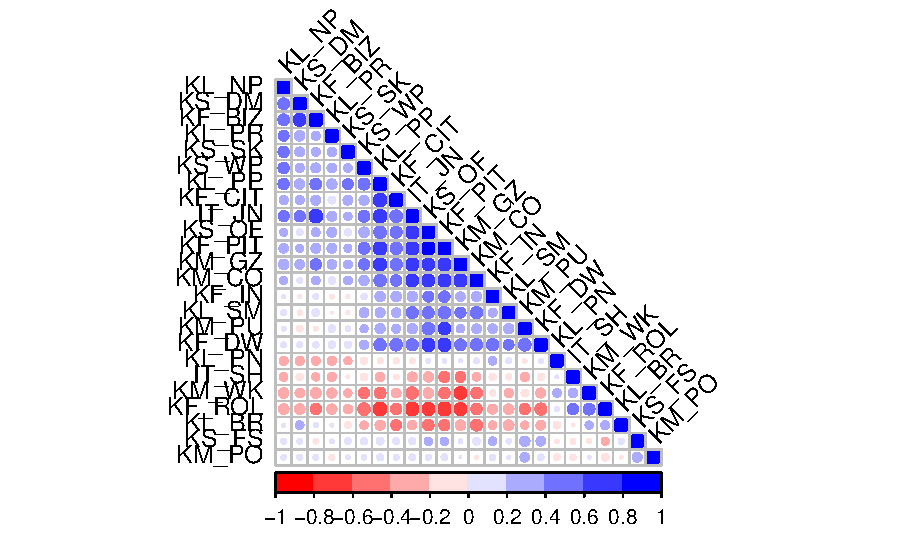
\includegraphics[width=1.3\linewidth]{figures/rycina1-1} 

}

\caption{Korelogram czynników diagnostycznych}\label{fig:rycina1}
\end{figure}

Zdecydowano się na współczynnik skolaryzacji netto dla szkół podstawowych mając na uwadze ciągłość danych, ponieważ reforma edukacyjna z 2019 roku zlikwidowała gimnazja.
Dodano wskaźnik podmioty gospodarcze w sekcjach J-N (usługi, specjaliści, informatyka) na 1000 mieszkańców, w celu zwiększenia liczby wskaźników stanowiących o innowacyjności danej jednostki przestrzennej.
W ten sposób powstały 24 zmienne diagnostyczne, które wykorzystano przy konstrukcji syntetycznego wskaźnika poziomu rozwoju dla lat 2016-2019 (Tabela \ref{tab:tabela1}).

\begin{table}

\caption{\label{tab:tabela1}Zmienne diagnostyczne, wykorzystane do konstrukcji syntetycznego wskaźnika rozwoju}
\centering
\begin{tabular}[t]{>{\raggedright\arraybackslash}p{2cm}>{\raggedright\arraybackslash}p{11cm}l}
\toprule
Skrot & Nazwa.wskaznika & Typ\\
\midrule
KL\_NP & ludność w wieku nieprod. na 100 w wieku prod. & Destymulanta\\
KL\_PN & przyrost naturalny na 1000 ludności w ‰ & Stymulanta\\
KL\_SM & saldo migracji ogółem na 1000 ludności & Stymulanta\\
KL\_PR & przychodnie na 10 tys. ludności & Stymulanta\\
KL\_BR & udział bezrobotnych zarejestrowanych w liczbie ludności w wieku produkcyjnym & Destymulanta\\
\addlinespace
KL\_PP & pracujący na 1000 osób w wieku produkcyjnym & Stymulanta\\
KS\_FS & fundacje, stowarz., organizacje na 1000 lub 10 tys. osób & Stymulanta\\
KS\_OF & osoby fizyczne prow. działalność gos. na 1000 ludności & Stymulanta\\
KS\_WP & udział przedstawicieli władz publicznych, wyższych urzędników, kierowników oraz specjalistów w ogóle radnych  [\%] & Stymulanta\\
KS\_SK & współczynnik skolaryzacji netto szkoły podstawowe & Stymulanta\\
\addlinespace
KS\_DM & liczba dodatków mieszkaniowych na 1000 mieszkańców - wskaźnik ubóstwa & Destymulanta\\
KM\_GZ & udział osób korzystających z instalacji gazowej w ogóle populacji [\%] & Stymulanta\\
KM\_PO & obszary prawnie chronione jako \% powierzchni gminy – wskaźnik posiadanych walorów środowiska & Stymulanta\\
KM\_WK & różnica pomiędzy odsetkiem ludności korzystającej z wodociągu i z kanalizacji wg lokalizacji & Destymulanta\\
KM\_PU & przeciętna powierzchnia użytkowa mieszkania na 1 osobę & Stymulanta\\
\addlinespace
KM\_CO & \% mieszkań posiadających centralne ogrzewanie & Stymulanta\\
KF\_IN & wydatki majątkowe inwestycyjne budżetów gmin i miast na prawach powiatu na 1 mieszkańca [zł/os.] & Stymulanta\\
KF\_PIT & dochody z podatku PIT na 1 mieszkańca [zł] & Stymulanta\\
KF\_CIT & dochody z podatku CIT na 1 mieszkańca [zł] & Stymulanta\\
KF\_ROL & dochody z podatku rolnego na 1 mieszkańca [zł] & Stymulanta\\
\addlinespace
KF\_DW & dochody własne per capita [zł] & Stymulanta\\
KF\_BIZ & instytucje otoczenia biznesu na 10 tys. podmiotów gospodarki narodowej & Stymulanta\\
IT\_SH & spółki handlowe z udziałem kapitału zagranicznego na 1000 podmiotów gospodarczych & Stymulanta\\
IT\_JN & podmioty gospodarcze w sekcjach J-N (usługi, specjalisci, informatyka) na 1000 mieszkańców & Stymulanta\\
\bottomrule
\multicolumn{3}{l}{\textsuperscript{*} Zródło: Opracowanie własne}\\
\end{tabular}
\end{table}

Dane obejmują lata 2016-2019, w tym czasie doszło do kilku ważnych zmian administracyjnych w województwie zachodniopomorskim, które miały wpływ podczas procesu przetwarzania danych.
W badanym okresie liczba gmin z 114 zmniejszyła się do 113.
Stało się tak, ponieważ w 2019 roku zlikwidowano gminę Ostrowice.
Przyczyną było bankructwo gminy- jest to pierwszy tego typu przypadek w Polsce.
Teren gminy Ostrowice został włączony do dwóch sąsiednich gmin, Drawska Pomorskiego i gminy Złocieniec.\autocite{ostrowice}
Z powodu problemów finansowych w gminie Ostrowice w latach 2017-2018 rada gminy nie istniała, a do zarządzania gminą został powołany przedstawiciel rządu.
Dlatego zdecydowano, że wskaźnik udziału przedstawicieli władz publicznych, wyższych urzędników, kierowników oraz specjalistów w ogóle radnych dla gminy Ostrowice w latach 2017-2018 będzie wynosił 0.
W badanym okresie gmina Mielno w 2017 przekształciła się z gminy wiejskiej na wiejsko-miejską, nie wpłynęło to jednak znacząco na proces badawczy.

\hypertarget{wskaznik}{%
\section{Konstrukcja syntetycznego miernika poziomu rozwoju społeczno-gospodarczego}\label{wskaznik}}

Do konstrukcji syntetycznych wskaźników rozwoju konieczne było przekształcenie zmiennych tak by były porównywalne. Dokonując wyboru metody pozwalającej na ujednolicenie rzędu wielkości zmiennych oraz pozbycia się mian kierowano się wykresem gęstości zmiennych. Ustalono, że większość zmiennych diagnostycznych cechuje się asymetrią prawostronną rozkładu (Rysunek \ref{fig:rycina2}).

\begin{figure}[t]

{\centering 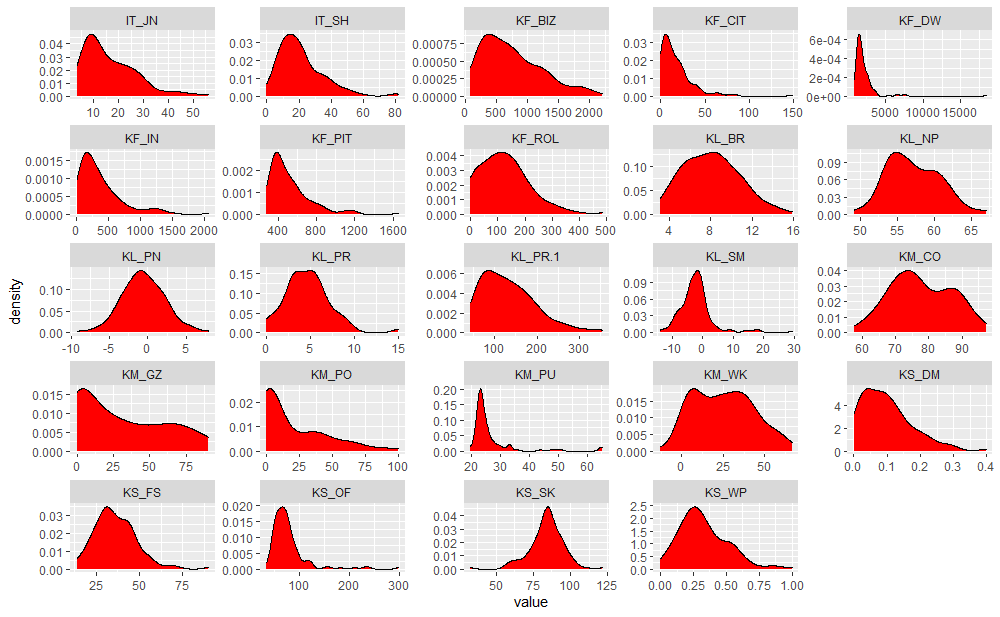
\includegraphics[width=1\linewidth]{figures/Gestosc_2016} 

}

\caption{Wykres estymatorów gęstości zmiennych diagnostycznych (2016)}\label{fig:rycina2}
\end{figure}

Mając na uwadze to że większość zmiennych nie charakteryzowało się rozkładem normalnym, zdecydowano się na metodę unitaryzacji zerowanej (za \textcite{churski_teoretyczny}).
Metoda ta wymaga następującej formuły dla:

\begin{itemize}
\tightlist
\item
  stymulanty
\end{itemize}

\[ 
Z_{ij} = \frac{X_{ij}-\min_{i}X_{ij}}{\max_{i}X_{ij}-\min_{i}X_{ij}}
\]

\begin{itemize}
\tightlist
\item
  destymulanty
\end{itemize}

\[ 
Z_{ij} = \frac{\max_{i}X_{ij}-X_{ij}}{\max_{i}X_{ij}-\min_{i}X_{ij}}
\]
Polega to na tym, że każda minimalna wartość danej zmiennej jest przekształcana na 0, maksymalna wartość jest przekształcana na 1, a każda inna wartość jest przekształcana na ułamek z zakresu od 0 do 1.
Dzięki zastosowaniu normalizacji zerowanej mamy pewność że wszystkie poddane normalizacji zmienne (także te ujemne) będą nieujemne i znajdowały się w tym samym przedziale (od 0 do 1).

Następnym krokiem jest konstrukcja syntetycznego wskaźnika rozwoju na bazie zunitaryzowanych wskaźników z wykorzystaniem metody wzorca rozwoju.
W metodzie tej transformowano miarę niepodobieństwa Braya-Curtisa na miarę podobieństwa do wzorca, gdzie jako wzorzec przyjęto hipotetyczną jednostkę przestrzenną, która przyjmowała wartość maksymalną dla wszystkich zmiennych diagnostycznych (za \textcite{perdal_zastosowanie})

\[ d_{kj}^{BC} = 1 - \frac{ \sum_{j=1}^{m} | Z_{ij} - Z_{kj}| } {\sum_{j=1}^{m} | Z_{ij} + Z_{kj}|  }\]
gdzie:
\(Z_{ij}\) - zunitaryzowana wartość wskaźnika \(j\) dla gminy \(i\)

\(k\) - gmina ``wzorzec''

\(j\in\{1,2,\dots,m\}\) - numer wskaźnika

Wskaźniki syntetyczne przyjmują wartość z przedziału {[}0,1{]}, im większa wartość wskaźnika syntetycznego rozwoju tym wyższy poziom rozwoju społeczno-gospodarczego. Syntetyczny wskaźnik poziomu rozwoju obejmuje wszystkie 24 zmienne diagnostyczne (Patrz Tabela \ref{tab:tabela1}). Wskaźniki syntetyczne wyróżnionych aspektów poziomu rozwoju społeczno-gospodarczego (tj. kapitał ludzki, materialny), obejmują określone w Tabeli \ref{tab:tabela1} wskaźniki diagnostyczne.

\hypertarget{metody}{%
\chapter{Metody analizy danych}\label{metody}}

\hypertarget{skupien}{%
\section{Analiza skupień - pojęcie, K-średnich, DBSCAN}\label{skupien}}

Analiza skupień jest ważnym elementem statystycznej analizy danych.
Pojęcie to pierwszy raz użyto w 1939 roku przez Roberta Choate Tryona w pracy \emph{cluster analysis} (za \textcite{najman}).
Analiza skupień polega na grupowaniu danych w grupy zwane tez skupieniami, w zależności od tego jak ściśle są ze sobą powiązane.
Dąży się do tego żeby dane w jednym skupieniu charakteryzowały się wysokim poziomem podobieństwa, natomiast dane między skupieniami miały minimalny poziom podobieństwa.
Obecnie istnieje wiele metod i technik analizy skupień, w niniejszej pracy opisano metodę K-średnich oraz metodę DBSCAN.

Metoda K-średnich należy do jednych z najczęściej stosowanych algorytmów analizy skupień.
W grupowaniu K-średnich każde skupienie jest reprezentowane przez swój środek (tj. centroid), który odpowiada średniej z obserwacji przypisanych do skupienia.
Istnieje kilka wariantów algorytmu dla tej metody, do najbardziej znanych należą (za \textcite{k-srednich_book}):

\begin{itemize}
\tightlist
\item
  Forgy/Lloyd
\item
  MacQueen
\item
  Hartigan-Wong
\end{itemize}

Standardowym oraz użytym w niniejszym badaniu algorytmem jest algorytm Hartigana-Wonga (1979), który definiuje całkowitą zmienność w obrębie skupienia jako sumę kwadratów odległości euklidesowych między elementami, a odpowiadającym im centroidem (za \textcite{k-srednich_internet}).

\[ W(C_k) = \sum_{{X_i}\in C_k}(X_i - \mu_k)^2
\]
gdzie:
\(X_i\) - obserwacja należąca do skupienia \(C_k\)

\(\mu_k\) - średnia wartość obserwacji przypisanych do skupienia \(C_k\)

Każda obserwacja (\(X_i\)) zostaje przypisana do określonego skupienia w taki sposób, że suma kwadratów odległości obserwacji do przypisywanego im centroidu (\(\mu_k\)) jest minimalna.
Całkowita suma kwadratów w obrębie skupienia jest definiowana wzorem:
\[ \sum_{k=1}^K W(C_k) = \sum_{k=1}^K \sum_{{X_i}\in C_k}(X_i - \mu_k)^2
\]
Im mniejsza wartość całkowitej sumy kwadratów tym lepiej.

Pierwszym krokiem przy wykorzystaniu algorytmu K-średnich jest wskazanie liczby skupień (\(k\)), które zostaną wygenerowane w ostatecznym rozwiązaniu.
Następnie algorytm losowo wybiera \(k\) obserwacji ze zbioru danych, które mają służyć jako początkowe centroidy dla skupień.
Każda z pozostałych obserwacji jest przypisywana do najbliższego centroidu, gdzie najbliższy jest definiowany za pomocą odległości euklidesowej:
\[ d (x,y) = \sqrt{\sum_{i=1}^n(X_i - Y_i)^2}
\]
między obserwacją a średnią skupień (przypisanie obserwacji do skupień).
W kolejnym kroku algorytm oblicza średnią wartość dla każdego skupienia (koryguje centroidy).
Wszystkie obserwacje są ponownie przypisywane przy użyciu skorygowanych centroidów.
Następnie powtarza się przypisanie obserwacji do skupień i korygowanie centroidów do momentu, aż przypisania do skupień przestaną się zmieniać.
Oznacza to, że skupienia utworzone w bieżącej iteracji są takie same, jak te uzyskane w poprzedniej iteracji.

Pierwszym krokiem w powyższym algorytmie jest wskazanie przez analityka liczby klastrów/skupień.
Przy wyborze optymalnej liczby klastrów oprócz wiedzy na temat charakteru danych warto kierować się jedną z metod służących do doboru liczby skupień.
W badaniu podczas wyboru optymalnej liczby skupień porównywano wyniki uzyskane trzema metodami:

\begin{itemize}
\tightlist
\item
  Metodą Łokcia (\emph{Elbow Method})
\item
  Metodą Średniego Zarysu (\emph{Average Silhouette Method})
\item
  Statystyczną Metodą Luki (\emph{Gap Statistic Method})
\end{itemize}

Metoda Łokcia polega na obliczeniu dla każdego \(k\) całkowitej sumy kwadratów wewnątrz klastra, a następnie przedstawienie na wykresie.
Można wyrazić ją wzorem:
\[ min(\sum^K_{k=1} W(C_k))
\]
Optymalna liczba klas występuje w miejscu zgięcia (kolana), czyli w gdzie \(k\) i liczba klas \(k>\) charakteryzuje się niską rozpiętością całkowitej sumy kwadratów wewnątrz skupienia.

Metoda Średniego Zarysu polega na wyliczeniu zarysu dla każdej obserwacji a~następnie współczynnika zarysu na podstawie średniej wartości zarysu (\(\overline{S}_k\)). Zarys wyraża się wzorem:
\[ S_i = \frac{b_i - a_i}{max(a_i , b_i)}
\]
gdzie:
\(a_i\) - średnia miara niepodobieństwa miedzy obserwacją a wszystkimi obserwacjami wewnątrz tego samego skupienia

\(b_i\) - najmniejsza średnia odległość do najbliższego skupienia, do którego nie należy \(a_i\)

Współczynnik zarysu wyraża się wzorem:
\[ SC = max_k\overline{S}_k
\]
gdzie:
\(\overline{S}_k\) - średnia wartość zarysu dla całego zbioru o k skupieniach

Statystyczną Metodą Luki została opracowana w 2001 roku przez R. Tibshirani, G. Walther, i T. Hastie (\textcite{gap}).
Wyraża się wzorem:
\[ Gap_n(k) = E^*_nlog(W_k)-log(W_k)
\]
gdzie:
\(E^*_n\) - oznacza wartość oczekiwaną przy wielkości próby \(n\) z rozkładu referencyjnego i jest zdefiniowane za pomocą metody bootstrap (\(B\)) poprzez wygenerowanie \(B\) kopii referencyjnych zbiorów danych i przez obliczenie średniej

\(W_k\) - macierz kowariancji wewnątrzgrupowych wtedy, gdy każda zmienna
oryginalna zastąpiona została zmienną wygenerowaną z rozkładu jednostajnego nad odcinkiem, który jest rozstępem próby zmiennej oryginalnej (za \textcite{korzeniewski})

Wybieramy liczbę skupień jako najmniejsze \(k\) takie, że:
\[Gap(k)\ge Gap(k+1)-S_{k+1.}
\]

DBSCAN (ang. \emph{Density-Based Spatial Clustering of Applications with Noise}) należy do algorytmów gęstościowych, czyli takich które biorą pod uwagę fakt, że skupienia są gęstymi grupami obserwacji.
Uproszczając chodzi o to, że jeśli konkretna obserwacja należy do skupienia to powinna znajdować się w pobliżu wielu innych obserwacji w tym skupieniu.

Najpierw wybieramy dwa parametry, maksymalny promień sąsiedztwa epsilon (\(\epsilon\)) i liczbę minimalnej liczby obserwacji, dla których możemy powiedzieć że tworzy skupienie (*minPts).
Następnie zaczynamy od wybrania dowolnej obserwacji w naszym zbiorze danych.
Jeśli w odległości \(\epsilon\) od tej obserwacji znajduje się więcej obserwacji niż wyznaczona minimalna liczba obserwacji dla skupienia, to uważamy obserwacje za część skupienia
Następnie rozszerzamy to skupienie, sprawdzając wszystkie nowe obserwacje i sprawdzając, czy one również mają więcej niż ustaloną minimalną liczbę obserwacji w odległości \(\epsilon\).
Gdy nie ma obserwacji spełniających nasze warunki wewnątrz skupienia to wybieramy nową dowolną obserwacje i powtarzamy algorytm.
Obserwacje, które w odległości \(\epsilon\) mają mniej niż minimalną liczbę obserwacji i nie są częścią żadnego skupienia uważamy za szum i nie przydzielamy do żadnego skupienia.
Sąsiedztwo \(\epsilon\)~obserwacji \(p\), oznaczone przez \(N\) wyraża się wzorem (za \textcite{dbscan}):
\[N_{Eps} (p)= \{{q\in D|dist(p,q) \le \epsilon}\}
\]

\hypertarget{klasyfikacja}{%
\section{Klasyfikacja - definicja, lasy losowe, xgboost}\label{klasyfikacja}}

Klasyfikacja to proces określenia przydziału obserwacji do jednej z predefiniowanych klas.
Każdą obserwację można oznaczyć parą \((x,y)\) gdzie \(x\) reprezentuje zbiór mierzonych cech, które mają mieć wpływ na etykietę klasy \(y\).
Problem klasyfikacji występuje, gdy trenujemy model w celu przewidzenia klasy \(y\) do jakiej należy obserwacja na podstawie cech obserwacji \(x\).
Elementem systemu klasyfikacji nadzorowanej jest próba ucząca (ang. \emph{learning sample}) składająca się z \(n\) niezależnych par zmiennych \((x_1,y_1),\dots,(x_n,y_n)\) (za \textcite{gorecki}).
Drugim elementem jest klasyfikator, który jest funkcją określona na przestrzeni wartości cech o wartościach w zbiorze etykiet skonstruowaną na bazie próby uczącej. Klasyfikator jest funkcją:
\[ d: X\rightarrow Y\]
Gdy obserwujemy nowy wektor \(X\) to prognozą etykiety \(Y\) jest \(d( X )\)
Kolejnym elementem jest ocena skuteczności działania klasyfikatora.
Ocenę wartości błędu klasyfikatora przeprowadza się na zbiorze testowych przykładów, dla których rzeczywista przynależność do klas jest znana i które nie są częścią zbioru uczącego.
Miarą jakości klasyfikatora \(d\)~jest rzeczywisty poziom błędu (za \textcite{gorecki}):
\[ e(d) = P(d(X)\not=Y)
\]
Błąd ten jest jednak niemożliwy do zmierzenia, ponieważ zazwyczaj rozkład pary \((X,Y)\) nie jest znany.
Dlatego opracowano metody oszacowania rzeczywistego poziomu błędu, które oparte są obliczaniu jakości klasyfikatora \(\hat d\) za pomocą warunkowego prawdopodobieństwie błędu, które ma postać:
\[ e(\hat{d})=P(\hat d(X)) \not = Y| {\displaystyle L}_n)
\]
gdzie:
\(e(\hat d)\) aktualny poziom błędu

\(L_n\) - losowa próba ucząca

\(L_n = \{(X_1,Y_1),\dots,(X_n,Y_n)\}\) jest ciągiem niezależnych par losowych o identycznym rozkładzie prawdopodobieństwa takim, jak rozkład pary \((X,Y)\)

Lasy losowe to metoda klasyfikacji nadzorowanej opracowana przez Leo Breimana w 2001 roku (za \textcite{perdal_zastosowanie}).
W założeniu metoda ma na celu modyfikacje klasycznych drzew klasyfikacyjnych poprzez dodanie przypadkowości za pomocą metody bootstrap.
Bootstrap to metoda która symuluje tworzenie wielu nowych zestawów danych poprzez pobieranie próbek z oryginalnych danych ze zwracaniem (patrz Rysunek \ref{fig:rycina3})

\begin{figure}[t]

{\centering 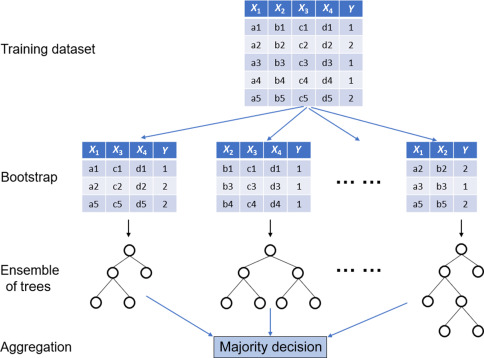
\includegraphics[width=1\linewidth]{figures/forest} 

}

\caption{Schemat algorytmu lasów losowych.                       Żródło:https://www.sciencedirect.com/topics/engineering/random-forest}\label{fig:rycina3}
\end{figure}

Dzięki tej modyfikacji lasy losowe w przeciwieństwie do drzew klasyfikacyjnych nie są tak wrażliwe na zmiany w danych uczących, a więc są bardziej odporne na błąd przeuczenia modelu.
Algorytm lasów losowych można przedstawić następująco (za \textcite{grzybowska}):

\begin{enumerate}
\def\labelenumi{\arabic{enumi}.}
\tightlist
\item
  Tworzymy \(N\) pseudo-próbek takich że \(S\in\{S_1,S_2,\dots,S_n\}\) poprzez pobieranie próbek ze zwracaniem
\item
  Dla każdego \(i\in\{1,2,\dots,N\}\) dokonywana jest losowa selekcja atrybutów ze zbioru uczącego \(X_*\) i budowany jest klasyfikator \(h_i = Learn(S_i;X_*)\)
\item
  Wynik uzyskiwany jest za pomocą reguły większościowej (ang. \emph{majority\textasciitilde vote})
\end{enumerate}

Metoda XGBoost czyli boosting gradientowy została opracowana w 1999 roku przez J. Fridmana (za \textcite{grzybowska}).
Konstruowana jest rodzina drzew, tak że następne drzewo tworzone jest na podstawie poprzedniego w kierunku wektora gradientu, dzięki czemu minimalizowana jest funkcja straty.
Algorytm XGBoost konstruowany w~następujący sposób (za \textcite{grzybowska}):

Niech \(Y = Learn(h(X))\) oraz \(b_m(X)\) będą predyktorami \(Y\)
\[ h(X) = \sum_{m=1}^Mb_m(x) = \sum_{m=1}^M\beta_mb(x;\theta_m)
\]
1. Podstawiamy: \[h_o(x) \leftarrow 0 \]
2. Dla \(m \in \{1,2,\dots,M\}\) i funkcji straty \(L()\):
\[r(x,y) \leftarrow - \frac{d}{dh}L(h_{m-1}(x),y)\]
\[b_m \leftarrow argmin_b\sum_{(x,y)}(b(x)-r(x,y))^2\]
\[h_m(X) \leftarrow h_{m-1}(x)+v*b_m(x)\]
W algorytmie tym wykorzystuje się fakt, że do zmiany \(h(x)\) na \(h(x)+vb(x)\) dla małych wartości \(v\) możemy użyć wyrażenia:
\[\sum_{(x,y)}L(h_{m-1}(x)+b_m(x),y) \approx \sum_{(x,y)}L(h_{m-1}(x),y)+\sum_{(x,y)}\frac {d}{dh}L(h_m-1(x)y)b_m(x)
\]

\hypertarget{wariancja}{%
\section{Analiza wariancji - jednoczynnikowa ANOVA, test Kruskala-Wallisa, testy post-hoc}\label{wariancja}}

Analiza wariancji to statystyczne narzędzie, które ma na celu porównanie wartości średnich zmiennej zależnej w analizowanych grupach wydzielonych ze względu na wartość zmiennych niezależnych.
Twórca analizy wariancji R. Fisher (za \textcite{wariancja}) wykazał, że większa różnica w średniej wartości zmiennej zależnej pomiędzy porównywanymi grupami przekłada się na większą wariancję międzygrupową.
Idea testu polega na rozłożeniu wariancji całkowitej na sumę wariancji międzygrupowych i wariancję wewnątrzgrupową (patrz Rysunek \ref{fig:rycina4}).

\begin{figure}[t]

{\centering 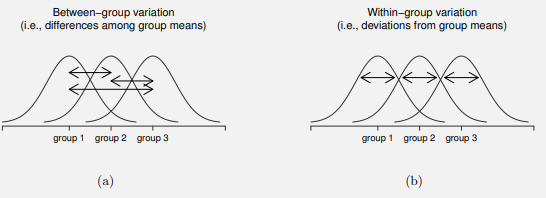
\includegraphics[width=1\linewidth]{figures/anova} 

}

\caption{Wariancje międzygrupowa (a) i wewnątrzgrupową (b)                              Źródło:https://stats.libretexts.org}\label{fig:rycina4}
\end{figure}

Hipoteza zerowa w teście analizy wariancji ma postać: \[H_0:\mu_1=\mu_2=\dots=\mu_L,\]
gdzie \(\mu_l\) jest wartością oczekiwaną w \(l\)-tej grupie, \(l=1,2,\dots,L\). Hipoteza alternatywna jest zaprzeczeniem hipotezy zerowej.

Jednoczynnikowa analiza wariancji (jednoczynnikowa \emph{ANOVA}) rozpatruje czy istnieją różnice w średnich wartościach ciągłej zmiennej zależnej w podgrupach wydzielonych ze względu na wartość zmiennej niezależnej.
Statystyka testowa przyjmuje postać (za \textcite{wariancja}):
\[ F=\frac{[\sum_{j=1}^K(\overline x_j - \overline x)^2n_j]/(k-1)}
{[\sum_{i=1}^{n_j}\sum_{j=1}^K(x_ij- \overline x_j)^2]/(n-k)}
\sim F(k-1,n-k)
\]
gdzie:
\(n_j\) - liczebności grup

\(\overline x_j\) - średnia w \(j\)-tej grupie

\(\overline x\) - średnia ogólna zmiennej zależnej

Powyższy rozkład jest prawdziwy przy prawdziwości hipotezy zerowej.

W przypadku przyjęcia hipotezy alternatywnej dla dokładniejszej analizy niezbędne są dodatkowe testy- tak zwane testy post-hoc (porównania wielokrotne).
W badaniu w~celu stwierdzenia jakie grupy istotnie różnią się między sobą wykonano test HSD Tukeya.

Test Kruskala-Wallisa został opracowany w 1952 roku.
Jest to test nieparametryczny (nie wymaga założeń odnośnie rozkładu populacji) będący alternatywą dla jednoczynnikowej analizy wariancji, która zakłada normalność cechy oraz homoskedastyczność wariancji.
Zakłada jednak, że rozkłady w grupach mają te same kształty.
Jest to test rangowy będący uogólnieniem testu Wilcoxona, obejmujący więcej niż dwie grupy, w~którym testuje się równość median.

Statystyka testowa wyraża się wzorem (za \textcite{kraskall}):
\[T=\frac{12}{n(n+1)}\sum_{i=1}^K\frac{R^2_i}{n_i}-3(n+1)
\]
gdzie:
\(R_i\) - suma rang w \(i\)-tej próbie

\(n_i\) - liczebność \(i\)-tej próby

\(n\) - łączna liczebność wszystkich grup

\hypertarget{ad}{%
\chapter{Analiza Danych}\label{ad}}

\hypertarget{miernik}{%
\section{Wyliczenie syntetycznego miernika rozwoju}\label{miernik}}

Analizę danych rozpoczęto od wczytania wstępnie oczyszczonych danych w formacie \emph{xlsx} za pomocą pakietu \emph{openxlsx} \autocite{R-openxlsx}.
Konstrukcje syntetycznego wskaźnika rozwoju rozpoczęto od wykonania funkcji unitaryzacji zerowanej (ang. \emph{min-max normalization}) dla wskaźników będących stymulantami lub destymulantami, za pomocą następujących instrukcji.

\begin{Shaded}
\begin{Highlighting}[]
\CommentTok{\#stymulanta}
\NormalTok{minmaxS }\OtherTok{\textless{}{-}} \ControlFlowTok{function}\NormalTok{(x, }\AttributeTok{na.rm =} \ConstantTok{FALSE}\NormalTok{) \{}
  \FunctionTok{return}\NormalTok{((x}\SpecialCharTok{{-}} \FunctionTok{min}\NormalTok{(x)) }\SpecialCharTok{/}\NormalTok{(}\FunctionTok{max}\NormalTok{(x)}\SpecialCharTok{{-}}\FunctionTok{min}\NormalTok{(x)))}
\NormalTok{\}}
\CommentTok{\#destymulanta}
\NormalTok{minmaxD }\OtherTok{\textless{}{-}} \ControlFlowTok{function}\NormalTok{(x, }\AttributeTok{na.rm =} \ConstantTok{FALSE}\NormalTok{) \{}
  \FunctionTok{return}\NormalTok{((}\FunctionTok{max}\NormalTok{(x)}\SpecialCharTok{{-}}\NormalTok{ x) }\SpecialCharTok{/}\NormalTok{(}\FunctionTok{max}\NormalTok{(x)}\SpecialCharTok{{-}}\FunctionTok{min}\NormalTok{(x)))}
\NormalTok{\}}
\end{Highlighting}
\end{Shaded}

Następnym krokiem było zastosowanie przygotowanej funkcji unitaryzacji zerowanej na danych dla odpowiednich wskaźników przy wykorzystaniu funkcji \emph{as.data.frame}, \emph{lapply} z pakietu \emph{base} \autocite{R-base} oraz \emph{select} z pakietu \emph{dplyr} \autocite{R-dplyr}.

\begin{Shaded}
\begin{Highlighting}[]
\FunctionTok{library}\NormalTok{(dplyr)}
\CommentTok{\#\textgreater{} }
\CommentTok{\#\textgreater{} Dołączanie pakietu: \textquotesingle{}dplyr\textquotesingle{}}
\CommentTok{\#\textgreater{} Następujący obiekt został zakryty z \textquotesingle{}package:kableExtra\textquotesingle{}:}
\CommentTok{\#\textgreater{} }
\CommentTok{\#\textgreater{}     group\_rows}
\CommentTok{\#\textgreater{} Następujące obiekty zostały zakryte z \textquotesingle{}package:stats\textquotesingle{}:}
\CommentTok{\#\textgreater{} }
\CommentTok{\#\textgreater{}     filter, lag}
\CommentTok{\#\textgreater{} Następujące obiekty zostały zakryte z \textquotesingle{}package:base\textquotesingle{}:}
\CommentTok{\#\textgreater{} }
\CommentTok{\#\textgreater{}     intersect, setdiff, setequal, union}
\CommentTok{\# wybieram i normalizuje stymulanty}
\NormalTok{gus2016\_normS }\OtherTok{\textless{}{-}} \FunctionTok{as.data.frame}\NormalTok{(}\FunctionTok{lapply}\NormalTok{(}\FunctionTok{select}\NormalTok{(Gus\_2016, }\DecValTok{4}\SpecialCharTok{:}\DecValTok{6}\NormalTok{, }\DecValTok{8}\SpecialCharTok{:}\DecValTok{12}\NormalTok{,}
    \DecValTok{14}\SpecialCharTok{:}\DecValTok{15}\NormalTok{, }\DecValTok{17}\SpecialCharTok{:}\DecValTok{26}\NormalTok{), minmaxS))}

\CommentTok{\# wybieram i normalizuje destymulanty}
\NormalTok{gus2016\_normD }\OtherTok{\textless{}{-}} \FunctionTok{as.data.frame}\NormalTok{(}\FunctionTok{lapply}\NormalTok{(}\FunctionTok{select}\NormalTok{(Gus\_2016, }\DecValTok{3}\NormalTok{, }\DecValTok{7}\NormalTok{,}
    \DecValTok{13}\NormalTok{, }\DecValTok{16}\NormalTok{), minmaxD))}

\CommentTok{\# łącze i dodaje TERYT, nazwa gminy}
\NormalTok{gus2016\_norm }\OtherTok{\textless{}{-}} \FunctionTok{cbind}\NormalTok{(gus2016\_normS, gus2016\_normD)}
\end{Highlighting}
\end{Shaded}

Następnie za pomocą następujących instrukcji skonstruowano i zastosowano funkcję opartą na mierze niepodobieństwa Braya-Curtisa (patrz Podrozdział \ref{wskaznik}) wyliczającą syntetyczny wskaźnik poziomu rozwoju oraz jego aspekty (patrz Podrozdział \ref{dane}).

\begin{Shaded}
\begin{Highlighting}[]
\FunctionTok{library}\NormalTok{(dplyr)}
\NormalTok{wskaznik }\OtherTok{\textless{}{-}} \ControlFlowTok{function}\NormalTok{(x) \{}
\NormalTok{  x\_abs }\OtherTok{\textless{}{-}} \FunctionTok{as.data.frame}\NormalTok{(}\FunctionTok{lapply}\NormalTok{(x, }\ControlFlowTok{function}\NormalTok{(y) }\FunctionTok{abs}\NormalTok{(y }\SpecialCharTok{{-}} \FunctionTok{max}\NormalTok{(y))))}
\NormalTok{  x\_sum }\OtherTok{\textless{}{-}} \FunctionTok{as.data.frame}\NormalTok{(}\FunctionTok{lapply}\NormalTok{(x, }\ControlFlowTok{function}\NormalTok{(y) y }\SpecialCharTok{+} \FunctionTok{max}\NormalTok{(y)))}
  \FunctionTok{return}\NormalTok{(}\DecValTok{1} \SpecialCharTok{{-}} \FunctionTok{rowSums}\NormalTok{(x\_abs) }\SpecialCharTok{/} \FunctionTok{rowSums}\NormalTok{(x\_sum))}
\NormalTok{\}}

\NormalTok{gus2016\_norm }\OtherTok{\textless{}{-}}\NormalTok{ gus2016\_norm }\SpecialCharTok{\%\textgreater{}\%}
  \FunctionTok{select}\NormalTok{(}\FunctionTok{order}\NormalTok{(}\FunctionTok{colnames}\NormalTok{(gus2016\_norm))) }\SpecialCharTok{\%\textgreater{}\%}
  \FunctionTok{mutate}\NormalTok{(}\AttributeTok{Rozwoj =} \FunctionTok{wskaznik}\NormalTok{(.),}
         \AttributeTok{K\_Ludzki =} \FunctionTok{wskaznik}\NormalTok{(}\FunctionTok{select}\NormalTok{(., }\DecValTok{9}\SpecialCharTok{:}\DecValTok{14}\NormalTok{)),}
         \AttributeTok{K\_Spoleczny =} \FunctionTok{wskaznik}\NormalTok{(}\FunctionTok{select}\NormalTok{(., }\DecValTok{20}\SpecialCharTok{:}\DecValTok{24}\NormalTok{)),}
         \AttributeTok{K\_Materialny =} \FunctionTok{wskaznik}\NormalTok{(}\FunctionTok{select}\NormalTok{(., }\DecValTok{15}\SpecialCharTok{:}\DecValTok{19}\NormalTok{)),}
         \AttributeTok{K\_Finansowy =} \FunctionTok{wskaznik}\NormalTok{(}\FunctionTok{select}\NormalTok{(., }\DecValTok{3}\SpecialCharTok{:}\DecValTok{8}\NormalTok{)),}
         \AttributeTok{Innowacje =} \FunctionTok{wskaznik}\NormalTok{(}\FunctionTok{select}\NormalTok{(., }\DecValTok{1}\SpecialCharTok{:}\DecValTok{2}\NormalTok{)))}
\end{Highlighting}
\end{Shaded}

Powstała ramka danych zawierająca wskaźnik syntetycznego poziomu rozwoju społeczno-gospodarczego i jego aspektów dla gmin w województwie Zachodniopomorskim w 2016 roku przedstawiała się następująco (patrz Tablica \ref{tab:tabela2}).
Analogicznie przeprowadzono unitaryzacje oraz obliczono syntetyczny wskaźnik rozwoju społeczno-gospodarczego oraz jego aspekty dla danych za rok 2017-2019.

\begin{table}

\caption{\label{tab:tabela2}Ramka danych dla wskaźnika syntetycznego poziomu rozwoju społeczno-gospodarczego i jego aspektów na przykładowych obserwacjach}
\centering
\resizebox{\linewidth}{!}{
\begin{tabular}[t]{lrrrrrr}
\toprule
  & Rozwoj & K\_Ludzki & K\_Spoleczny & K\_Materialny & K\_Finansowy & Innowacje\\
\midrule
Białogard (1) & 0.5271442 & 0.6075089 & 0.6007241 & 0.5272582 & 0.3664491 & 0.5127502\\
Białogard (2) & 0.3540260 & 0.4667454 & 0.5075338 & 0.2969588 & 0.1483996 & 0.2475569\\
Karlino (3) & 0.5041937 & 0.5668628 & 0.4540023 & 0.4760860 & 0.4708909 & 0.5907579\\
Tychowo (3) & 0.3803655 & 0.4953640 & 0.5466270 & 0.2702022 & 0.2395358 & 0.1676706\\
Bierzwnik (2) & 0.4312479 & 0.4574030 & 0.6481029 & 0.4503713 & 0.1981006 & 0.2673995\\
\addlinespace
Choszczno (3) & 0.5403547 & 0.5786519 & 0.5921272 & 0.6861926 & 0.3077595 & 0.4828032\\
\bottomrule
\multicolumn{7}{l}{\textsuperscript{*} Zródło: Opracowanie własne}\\
\end{tabular}}
\end{table}

\hypertarget{as_ad}{%
\section{Analiza skupień}\label{as_ad}}

Analizę skupień metodą K-średnich rozpoczęto od znalezienia optymalnej liczby skupień. Skorzystano z pakietu \emph{factoextra} (\textcite{R-factoextra}) i następującymi instrukcjami wykorzystując funkcję \emph{fviz\_nbclust}. Wykresy przedstawiające optymalną liczbę skupień wykonano dla każdego rocznika z przedziału 2016-2019 z pomocą pakietu \emph{ggplot2} (\textcite{R-ggplot2}) oraz połączono je za pomocą funkcji \emph{grid.arrange} z~pakietu \emph{gridExtra} (\textcite{R-gridExtra})

\begin{Shaded}
\begin{Highlighting}[]
\CommentTok{\# szukanie optymalnej liczby skupień Elbow Method}
\FunctionTok{set.seed}\NormalTok{(}\DecValTok{123}\NormalTok{)}
\NormalTok{p1 }\OtherTok{\textless{}{-}}\NormalTok{ factoextra}\SpecialCharTok{::}\FunctionTok{fviz\_nbclust}\NormalTok{(gus2016\_norm, kmeans, }\AttributeTok{method =} \StringTok{"wss"}\NormalTok{,}
    \AttributeTok{k.max =} \DecValTok{10}\NormalTok{) }\SpecialCharTok{+}\NormalTok{ ggplot2}\SpecialCharTok{::}\FunctionTok{geom\_vline}\NormalTok{(}\AttributeTok{xintercept =} \DecValTok{4}\NormalTok{, }\AttributeTok{linetype =} \DecValTok{2}\NormalTok{) }\SpecialCharTok{+}
\NormalTok{    ggplot2}\SpecialCharTok{::}\FunctionTok{ggtitle}\NormalTok{(}\StringTok{"2016"}\NormalTok{)}
\NormalTok{p2 }\OtherTok{\textless{}{-}}\NormalTok{ factoextra}\SpecialCharTok{::}\FunctionTok{fviz\_nbclust}\NormalTok{(gus2017\_norm, kmeans, }\AttributeTok{method =} \StringTok{"wss"}\NormalTok{,}
    \AttributeTok{k.max =} \DecValTok{10}\NormalTok{) }\SpecialCharTok{+}\NormalTok{ ggplot2}\SpecialCharTok{::}\FunctionTok{geom\_vline}\NormalTok{(}\AttributeTok{xintercept =} \DecValTok{4}\NormalTok{, }\AttributeTok{linetype =} \DecValTok{2}\NormalTok{) }\SpecialCharTok{+}
\NormalTok{    ggplot2}\SpecialCharTok{::}\FunctionTok{ggtitle}\NormalTok{(}\StringTok{"2017"}\NormalTok{)}
\NormalTok{p3 }\OtherTok{\textless{}{-}}\NormalTok{ factoextra}\SpecialCharTok{::}\FunctionTok{fviz\_nbclust}\NormalTok{(gus2018\_norm, kmeans, }\AttributeTok{method =} \StringTok{"wss"}\NormalTok{,}
    \AttributeTok{k.max =} \DecValTok{10}\NormalTok{) }\SpecialCharTok{+}\NormalTok{ ggplot2}\SpecialCharTok{::}\FunctionTok{geom\_vline}\NormalTok{(}\AttributeTok{xintercept =} \DecValTok{4}\NormalTok{, }\AttributeTok{linetype =} \DecValTok{2}\NormalTok{) }\SpecialCharTok{+}
\NormalTok{    ggplot2}\SpecialCharTok{::}\FunctionTok{ggtitle}\NormalTok{(}\StringTok{"2018"}\NormalTok{)}
\NormalTok{p4 }\OtherTok{\textless{}{-}}\NormalTok{ factoextra}\SpecialCharTok{::}\FunctionTok{fviz\_nbclust}\NormalTok{(gus2019\_norm, kmeans, }\AttributeTok{method =} \StringTok{"wss"}\NormalTok{,}
    \AttributeTok{k.max =} \DecValTok{10}\NormalTok{) }\SpecialCharTok{+}\NormalTok{ ggplot2}\SpecialCharTok{::}\FunctionTok{geom\_vline}\NormalTok{(}\AttributeTok{xintercept =} \DecValTok{4}\NormalTok{, }\AttributeTok{linetype =} \DecValTok{2}\NormalTok{) }\SpecialCharTok{+}
\NormalTok{    ggplot2}\SpecialCharTok{::}\FunctionTok{ggtitle}\NormalTok{(}\StringTok{"2019"}\NormalTok{)}

\NormalTok{gridExtra}\SpecialCharTok{::}\FunctionTok{grid.arrange}\NormalTok{(p1, p2, p3, p4)}
\end{Highlighting}
\end{Shaded}

\begin{center}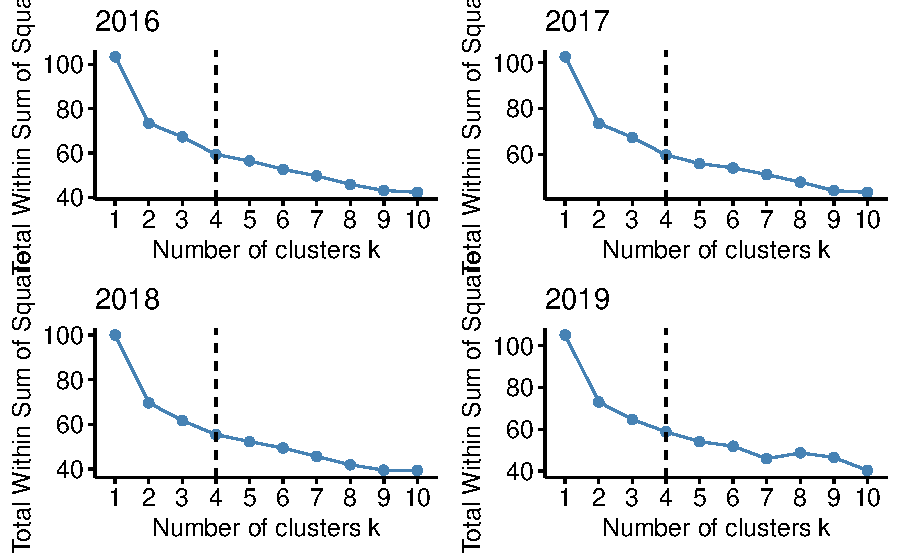
\includegraphics[width=1\linewidth]{figures/unnamed-chunk-9-1} \end{center}

W przypadku metody Łokcia, optymalną liczbę skupień wyznacza miejsce zgięcia (patrz Podrozdział \ref{skupien}). W tym przypadku dla danych za rok 2016 optymalna liczba skupień (\(k\)) to 4. Metoda Łokcia dla innych roczników wyznaczała taką samą optymalną liczbę skupień (4).

\begin{Shaded}
\begin{Highlighting}[]
\CommentTok{\# szukanie optymalnej liczby skupień Average Silhouette}
\CommentTok{\# Method}
\NormalTok{p1 }\OtherTok{\textless{}{-}}\NormalTok{ factoextra}\SpecialCharTok{::}\FunctionTok{fviz\_nbclust}\NormalTok{(gus2016\_norm, kmeans, }\AttributeTok{method =} \StringTok{"silhouette"}\NormalTok{) }\SpecialCharTok{+}
\NormalTok{    ggplot2}\SpecialCharTok{::}\FunctionTok{ggtitle}\NormalTok{(}\StringTok{"2016"}\NormalTok{)  }\CommentTok{\#idealnie 2, do 5 jest ok}
\NormalTok{p2 }\OtherTok{\textless{}{-}}\NormalTok{ factoextra}\SpecialCharTok{::}\FunctionTok{fviz\_nbclust}\NormalTok{(gus2017\_norm, kmeans, }\AttributeTok{method =} \StringTok{"silhouette"}\NormalTok{) }\SpecialCharTok{+}
\NormalTok{    ggplot2}\SpecialCharTok{::}\FunctionTok{ggtitle}\NormalTok{(}\StringTok{"2017"}\NormalTok{)  }\CommentTok{\#idealnie 2, do 5 jest ok}
\NormalTok{p3 }\OtherTok{\textless{}{-}}\NormalTok{ factoextra}\SpecialCharTok{::}\FunctionTok{fviz\_nbclust}\NormalTok{(gus2018\_norm, kmeans, }\AttributeTok{method =} \StringTok{"silhouette"}\NormalTok{) }\SpecialCharTok{+}
\NormalTok{    ggplot2}\SpecialCharTok{::}\FunctionTok{ggtitle}\NormalTok{(}\StringTok{"2018"}\NormalTok{)  }\CommentTok{\#idealnie 2, do 5 jest ok}
\NormalTok{p4 }\OtherTok{\textless{}{-}}\NormalTok{ factoextra}\SpecialCharTok{::}\FunctionTok{fviz\_nbclust}\NormalTok{(gus2019\_norm, kmeans, }\AttributeTok{method =} \StringTok{"silhouette"}\NormalTok{) }\SpecialCharTok{+}
\NormalTok{    ggplot2}\SpecialCharTok{::}\FunctionTok{ggtitle}\NormalTok{(}\StringTok{"2019"}\NormalTok{)}

\NormalTok{gridExtra}\SpecialCharTok{::}\FunctionTok{grid.arrange}\NormalTok{(p1, p2, p3, p4)}
\end{Highlighting}
\end{Shaded}

\begin{center}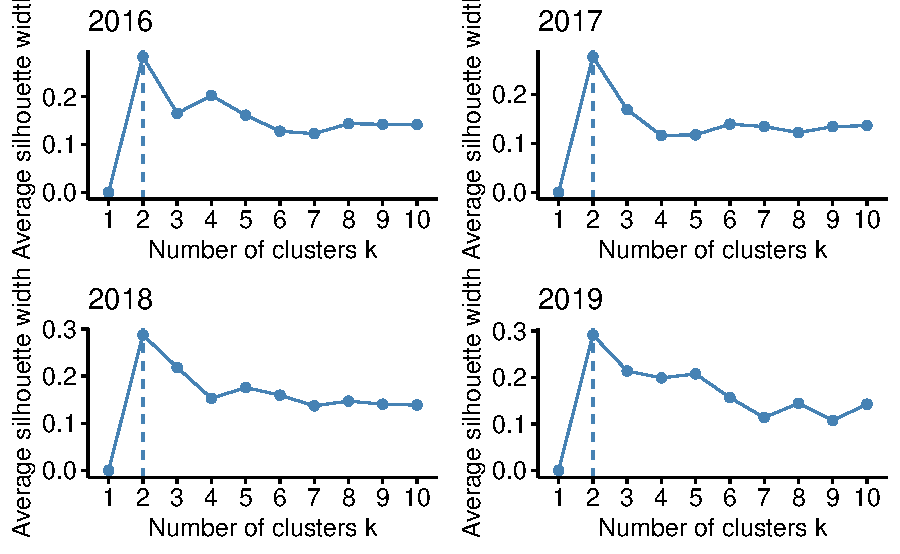
\includegraphics[width=1\linewidth]{figures/unnamed-chunk-10-1} \end{center}

W przypadku metody średniego zarysu (Average Silhouette Method) im większa wartość średniego zarysu dla danej liczby skupień \(k\) tym bardziej jest ona optymalna.
Jak widać optymalna liczba skupień we wszystkich latach to 2, jednak warto zauważyć, że średnia wartość zarysu dla 3 skupień jest niewiele mniejsza, zwłaszcza dla lat 2017-2019.

\begin{Shaded}
\begin{Highlighting}[]
\CommentTok{\# szukanie optymalnej liczby skupień Gap Statistic Method}
\NormalTok{p1 }\OtherTok{\textless{}{-}}\NormalTok{ factoextra}\SpecialCharTok{::}\FunctionTok{fviz\_nbclust}\NormalTok{(gus2016\_base, kmeans, }\AttributeTok{method =} \StringTok{"gap\_stat"}\NormalTok{) }\SpecialCharTok{+}
\NormalTok{    ggplot2}\SpecialCharTok{::}\FunctionTok{ggtitle}\NormalTok{(}\StringTok{"2016"}\NormalTok{)}
\NormalTok{p2 }\OtherTok{\textless{}{-}}\NormalTok{ factoextra}\SpecialCharTok{::}\FunctionTok{fviz\_nbclust}\NormalTok{(gus2017\_norm, kmeans, }\AttributeTok{method =} \StringTok{"gap\_stat"}\NormalTok{) }\SpecialCharTok{+}
\NormalTok{    ggplot2}\SpecialCharTok{::}\FunctionTok{ggtitle}\NormalTok{(}\StringTok{"2017"}\NormalTok{)}
\NormalTok{p3 }\OtherTok{\textless{}{-}}\NormalTok{ factoextra}\SpecialCharTok{::}\FunctionTok{fviz\_nbclust}\NormalTok{(gus2018\_norm, kmeans, }\AttributeTok{method =} \StringTok{"gap\_stat"}\NormalTok{) }\SpecialCharTok{+}
\NormalTok{    ggplot2}\SpecialCharTok{::}\FunctionTok{ggtitle}\NormalTok{(}\StringTok{"2018"}\NormalTok{)}
\NormalTok{p4 }\OtherTok{\textless{}{-}}\NormalTok{ factoextra}\SpecialCharTok{::}\FunctionTok{fviz\_nbclust}\NormalTok{(gus2019\_norm, kmeans, }\AttributeTok{method =} \StringTok{"gap\_stat"}\NormalTok{) }\SpecialCharTok{+}
\NormalTok{    ggplot2}\SpecialCharTok{::}\FunctionTok{ggtitle}\NormalTok{(}\StringTok{"2019"}\NormalTok{)}

\NormalTok{gridExtra}\SpecialCharTok{::}\FunctionTok{grid.arrange}\NormalTok{(p1, p2, p3, p4)}
\end{Highlighting}
\end{Shaded}

\begin{center}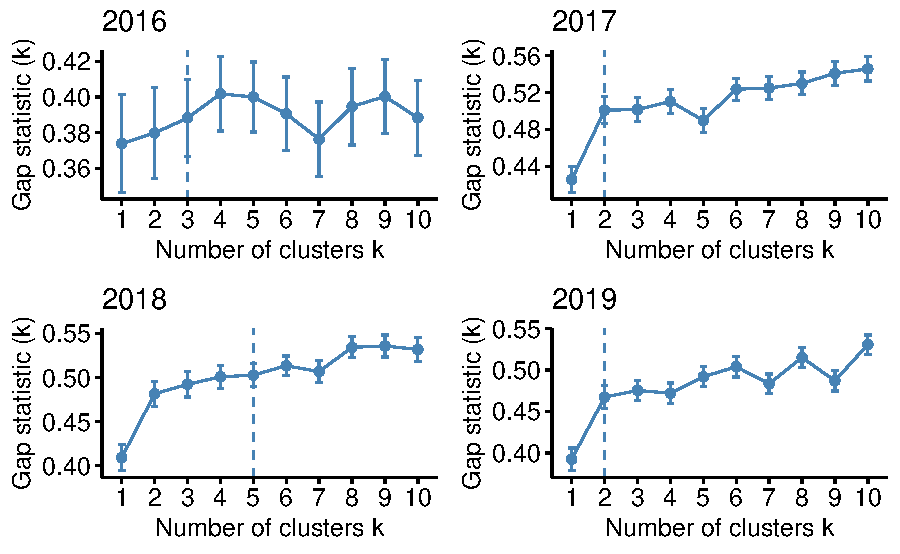
\includegraphics[width=1\linewidth]{figures/unnamed-chunk-11-1} \end{center}

Dla statystycznej metody luki (Gap Statistic Method) optymalna liczba skupień \(k\) to taka, dla której wartość statystyki luki jest większa niż \(k+1\) minus odchylenie standardowe. Co ciekawe dla różnych roczników statystyka ta przyjmuje różne wartości. Dla 2016 roku optymalna liczba skupień to 3, dla 2017, 2019 roku optymalną liczbą skupień to 2, natomiast dla 2018 roku optymalna liczba skupień to 5.

Ostatecznie kierując się powyższymi statystykami, sprawdzając jak rozkładają się obserwacje dla różnej liczby skupień i kierując się wiedzą merytoryczną z zakresu badań nad poziomem rozwoju oraz praktyką badawczą, sugerującą nieparzystą i ograniczoną liczbę skupień zdecydowano się na dalsze badania dla 3 skupień. Natomiast warto zaznaczyć, że liczby skupień 4 lub 5 wydają się też dość optymalne. W badaniach Pana Doktora Perdała (\textcite{perdal_zastosowanie}) za optymalna liczbę skupień określono 5.

Przydzielanie do skupień metodą K-średnich wykonano za pomocą następujących instrukcji korzystając z funkcji \emph{kmeans} oraz \emph{fviz\_cluster} z pakietu \emph{factoExtra} (\textcite{R-factoExtra}).
W funkcji \emph{fviz\_cluster} obserwacje są reprezentowane przez punkty na wykresie, przy użyciu dwóch pierwszych składowych głównych.

\begin{Shaded}
\begin{Highlighting}[]
\NormalTok{k1 }\OtherTok{\textless{}{-}} \FunctionTok{kmeans}\NormalTok{(gus2016\_base}\SpecialCharTok{$}\NormalTok{Rozwoj, }\AttributeTok{centers =} \DecValTok{3}\NormalTok{, }\AttributeTok{nstart =} \DecValTok{10}\NormalTok{)}
\NormalTok{factoextra}\SpecialCharTok{::}\FunctionTok{fviz\_cluster}\NormalTok{(k1, }\AttributeTok{data =}\NormalTok{ gus2016\_base) }\SpecialCharTok{+}\NormalTok{ ggplot2}\SpecialCharTok{::}\FunctionTok{ggtitle}\NormalTok{(}\StringTok{"2016"}\NormalTok{)}
\end{Highlighting}
\end{Shaded}

\begin{center}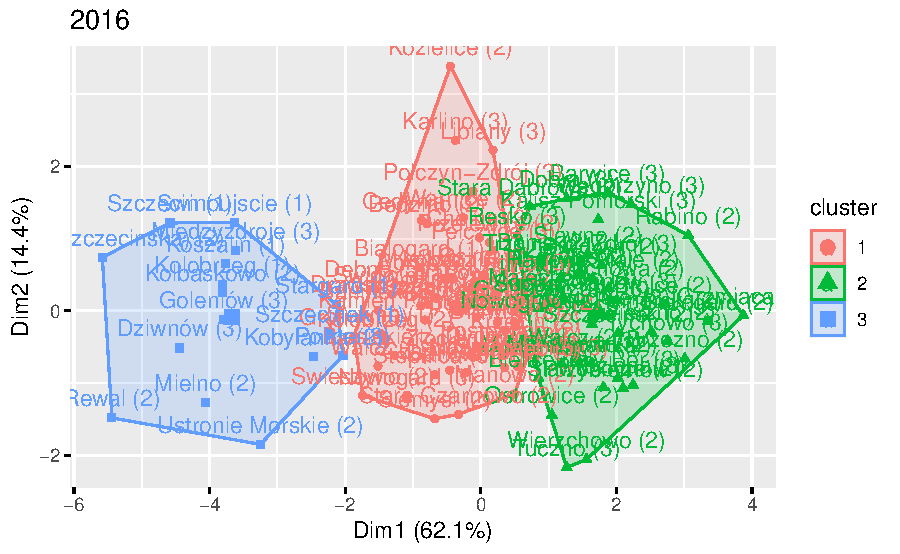
\includegraphics[width=1.05\linewidth]{figures/rycina5 -1} \end{center}

Interpretacja skupień dla obserwacji z 2016 roku przedstawia się następująco (dokładane przedstawienie poziomów rozwoju dla poszczególnych obserwacji w Podrozdziale (\ref{mapy})):

\begin{itemize}
\tightlist
\item
  skupienie o numeracji 1 przedstawia obserwacje o średnim poziomie rozwoju
\item
  skupienie o numeracji 2 przedstawia obserwacje o niskim poziomie rozwoju
\item
  skupienie o numeracji 3 przedstawia obserwacje o wysokim poziomie rozwoju
\end{itemize}

\begin{Shaded}
\begin{Highlighting}[]
\NormalTok{k2 }\OtherTok{\textless{}{-}} \FunctionTok{kmeans}\NormalTok{(gus2017\_base}\SpecialCharTok{$}\NormalTok{Rozwoj, }\AttributeTok{centers =} \DecValTok{3}\NormalTok{, }\AttributeTok{nstart =} \DecValTok{10}\NormalTok{)}
\NormalTok{factoextra}\SpecialCharTok{::}\FunctionTok{fviz\_cluster}\NormalTok{(k2, }\AttributeTok{data =}\NormalTok{ gus2017\_base) }\SpecialCharTok{+}\NormalTok{ ggplot2}\SpecialCharTok{::}\FunctionTok{ggtitle}\NormalTok{(}\StringTok{"2017"}\NormalTok{)}
\end{Highlighting}
\end{Shaded}

\begin{center}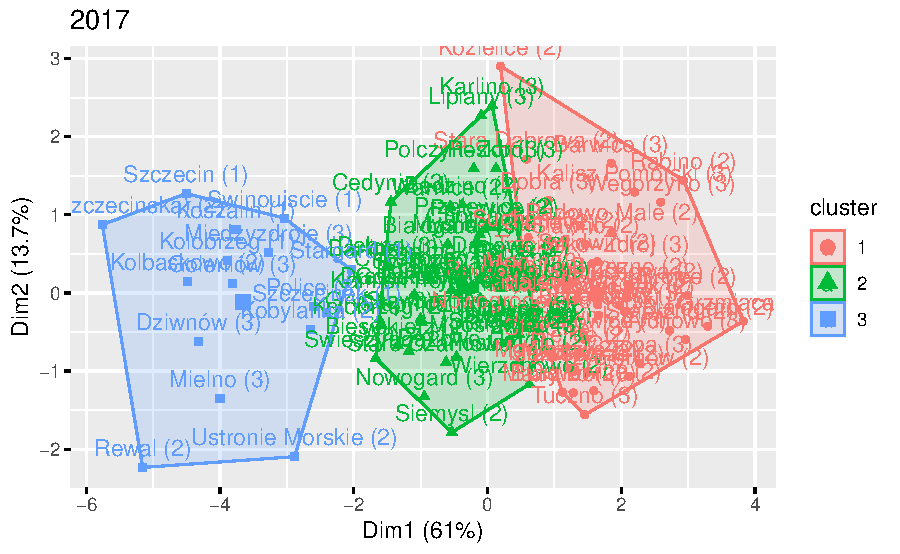
\includegraphics[width=1.05\linewidth]{figures/unnamed-chunk-12-1} \end{center}

Interpretacja skupień dla obserwacji z 2017 roku przedstawia się następująco:

\begin{itemize}
\tightlist
\item
  skupienie o numeracji 1 przedstawia obserwacje o średnim poziomie rozwoju
\item
  skupienie o numeracji 2 przedstawia obserwacje o niskim poziomie rozwoju
\item
  skupienie o numeracji 3 przedstawia obserwacje o wysokim poziomie rozwoju
\end{itemize}

\begin{Shaded}
\begin{Highlighting}[]
\NormalTok{k3 }\OtherTok{\textless{}{-}} \FunctionTok{kmeans}\NormalTok{(gus2018\_base}\SpecialCharTok{$}\NormalTok{Rozwoj, }\AttributeTok{centers =} \DecValTok{3}\NormalTok{, }\AttributeTok{nstart =} \DecValTok{10}\NormalTok{)}
\NormalTok{factoextra}\SpecialCharTok{::}\FunctionTok{fviz\_cluster}\NormalTok{(k3, }\AttributeTok{data =}\NormalTok{ gus2018\_base) }\SpecialCharTok{+}\NormalTok{ ggplot2}\SpecialCharTok{::}\FunctionTok{ggtitle}\NormalTok{(}\StringTok{"2018"}\NormalTok{)}
\end{Highlighting}
\end{Shaded}

\begin{center}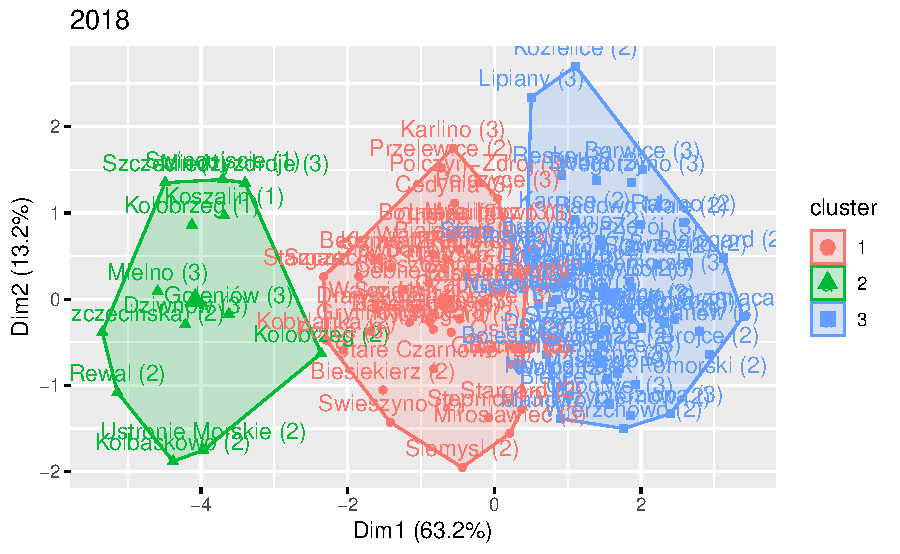
\includegraphics[width=1.05\linewidth]{figures/unnamed-chunk-13-1} \end{center}

Interpretacja skupień dla obserwacji z 2018 roku przedstawia się następująco:

\begin{itemize}
\tightlist
\item
  skupienie o numeracji 1 przedstawia obserwacje o średnim poziomie rozwoju
\item
  skupienie o numeracji 2 przedstawia obserwacje o wysokim poziomie rozwoju
\item
  skupienie o numeracji 3 przedstawia obserwacje o niskim poziomie rozwoju
\end{itemize}

\begin{Shaded}
\begin{Highlighting}[]
\NormalTok{k4 }\OtherTok{\textless{}{-}} \FunctionTok{kmeans}\NormalTok{(gus2019\_base}\SpecialCharTok{$}\NormalTok{Rozwoj, }\AttributeTok{centers =} \DecValTok{3}\NormalTok{, }\AttributeTok{nstart =} \DecValTok{10}\NormalTok{)}
\NormalTok{factoextra}\SpecialCharTok{::}\FunctionTok{fviz\_cluster}\NormalTok{(k4, }\AttributeTok{data =}\NormalTok{ gus2019\_base) }\SpecialCharTok{+}\NormalTok{ ggplot2}\SpecialCharTok{::}\FunctionTok{ggtitle}\NormalTok{(}\StringTok{"2019"}\NormalTok{)}
\end{Highlighting}
\end{Shaded}

\begin{center}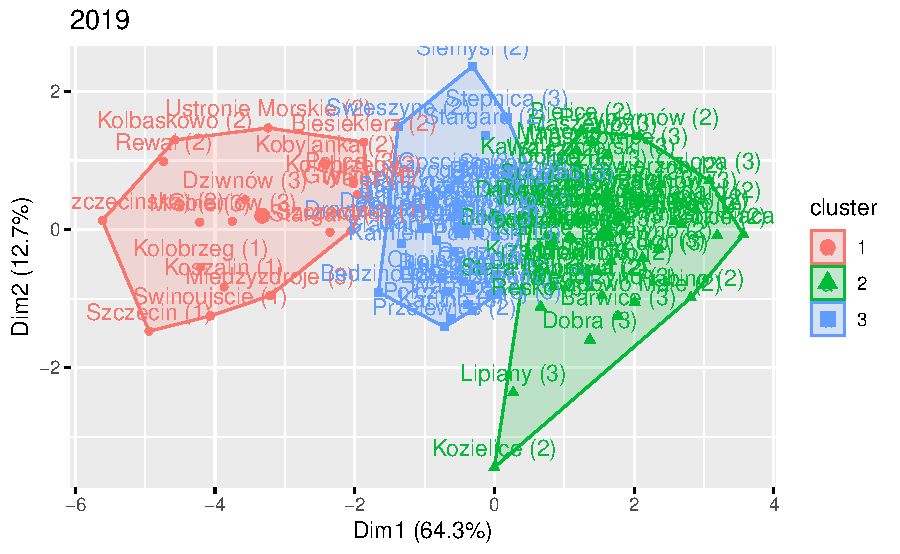
\includegraphics[width=1.05\linewidth]{figures/unnamed-chunk-14-1} \end{center}

Interpretacja skupień dla obserwacji z 2019 roku przedstawia się następująco:

\begin{itemize}
\tightlist
\item
  skupienie o numeracji 1 przedstawia obserwacje o wysokim poziomie rozwoju
\item
  skupienie o numeracji 2 przedstawia obserwacje o niskim poziomie rozwoju
\item
  skupienie o numeracji 3 przedstawia obserwacje o średnim poziomie rozwoju
\end{itemize}

Jak widać na powyższych wykresach, liczba skupień 3 dla metody K-średnich wygląda zadowalająco. Także, metoda K-średnich dla podziału obserwacji ze względu na syntetyczny wskaźnik poziomu rozwoju wydaje się optymalna.

W celu porównania wyników grupowania skupień za pomocą innej metody niż K-średnich zdecydowano się na wykonanie analizy DBSCAN. Analizę skupień metodą DBSCAN wykonano za pomocą pakietu \emph{dbscan} (\textcite{R-dbscan}).
Rozpoczęto od oszacowania wartości \(\epsilon\) za pomocą funkcji \emph{kNNdistplot}, która polega na obliczeniu i wyrysowaniu K-najbliższych odległości.
Następnie analityk określa moment zgięcia (kolana), który odpowiada optymalnemu parametrowi \(\epsilon\).

\begin{Shaded}
\begin{Highlighting}[]
\NormalTok{dbscan}\SpecialCharTok{::}\FunctionTok{kNNdistplot}\NormalTok{(gus2016\_base, }\AttributeTok{k =} \DecValTok{3}\NormalTok{)}
\FunctionTok{abline}\NormalTok{(}\AttributeTok{h =} \FloatTok{0.135}\NormalTok{, }\AttributeTok{lty =} \DecValTok{2}\NormalTok{)}
\FunctionTok{set.seed}\NormalTok{(}\DecValTok{12345}\NormalTok{)}
\NormalTok{model.dbscan }\OtherTok{\textless{}{-}}\NormalTok{ fpc}\SpecialCharTok{::}\FunctionTok{dbscan}\NormalTok{(gus2016\_base, }\AttributeTok{eps =} \FloatTok{0.175}\NormalTok{, }\AttributeTok{MinPts =} \DecValTok{2}\NormalTok{)}
\NormalTok{factoextra}\SpecialCharTok{::}\FunctionTok{fviz\_cluster}\NormalTok{(model.dbscan, gus2016\_base, }\AttributeTok{geom =} \StringTok{"point"}\NormalTok{)}
\end{Highlighting}
\end{Shaded}

\begin{center}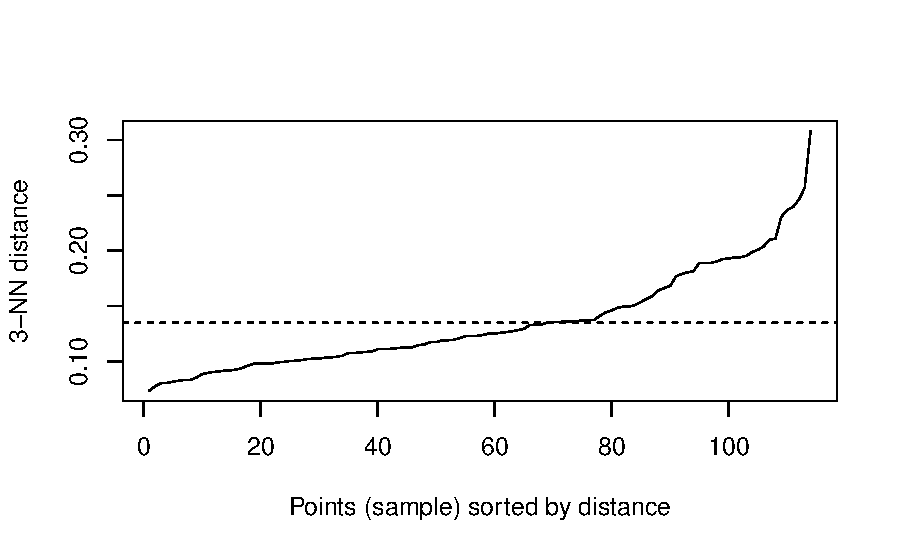
\includegraphics[width=1\linewidth]{figures/unnamed-chunk-15-1} 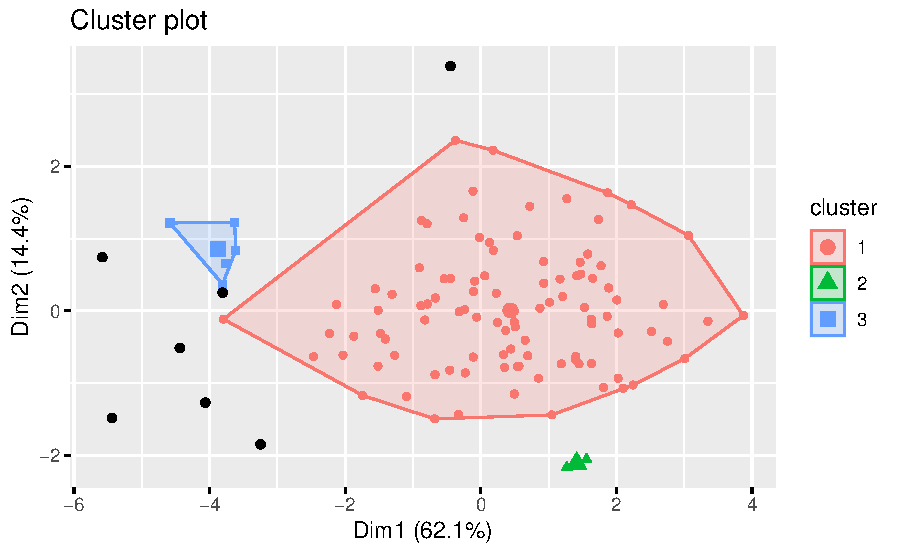
\includegraphics[width=1\linewidth]{figures/unnamed-chunk-15-2} \end{center}

Jak widać powyżej dla badanych obserwacji metoda DBSCAN nie daje satysfakcjonujących wyników z uwagi na przydzielenie wielu obserwacji do szumu, co w przypadku, gdy obserwacjami są gminy jest niezasadne merytorycznie. Dlatego pewnym rozwinięciem metody DBSCAN jest metoda OPTICS, w której efekty grupowania są podobne jak w~DBSCAN, z tą różnicą, że metoda ta nie zostawia obserwacji bez przypisanego skupienia (szumu).

\begin{Shaded}
\begin{Highlighting}[]
\CommentTok{\# Model optics, Reachability plot}
\NormalTok{model.optics }\OtherTok{\textless{}{-}}\NormalTok{ dbscan}\SpecialCharTok{::}\FunctionTok{optics}\NormalTok{(gus2016\_base, }\AttributeTok{eps =} \FloatTok{0.175}\NormalTok{, }\AttributeTok{minPts =} \DecValTok{2}\NormalTok{)}
\FunctionTok{plot}\NormalTok{(model.optics)}
\end{Highlighting}
\end{Shaded}

\begin{center}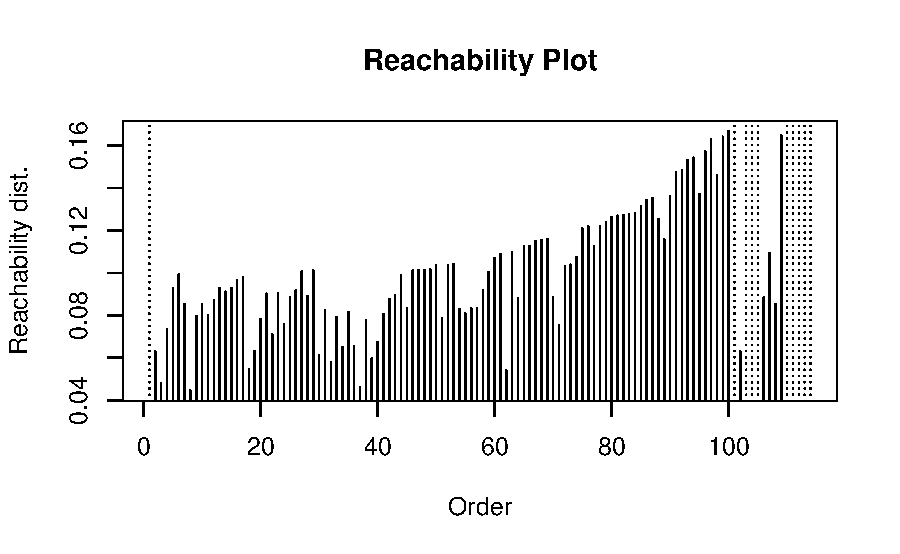
\includegraphics[width=1\linewidth]{figures/unnamed-chunk-16-1} \end{center}

Doliny na wykresie dostępności informują o istnieniu skupień, a szerokość doliny informuje o licznie obiektów przydzielonych do różnych skupień.

\begin{Shaded}
\begin{Highlighting}[]
\CommentTok{\# optics skupienia}
\NormalTok{(result.optics }\OtherTok{\textless{}{-}}\NormalTok{ dbscan}\SpecialCharTok{::}\FunctionTok{extractDBSCAN}\NormalTok{(model.optics, }\AttributeTok{eps\_cl =} \FloatTok{0.4}\NormalTok{))}
\CommentTok{\#\textgreater{} OPTICS ordering/clustering for 114 objects.}
\CommentTok{\#\textgreater{} Parameters: minPts = 2, eps = 0.175, eps\_cl = 0.4, xi = NA}
\CommentTok{\#\textgreater{} The clustering contains 3 cluster(s) and 7 noise points.}
\CommentTok{\#\textgreater{} }
\CommentTok{\#\textgreater{}   0   1   2   3 }
\CommentTok{\#\textgreater{}   7 100   2   5 }
\CommentTok{\#\textgreater{} }
\CommentTok{\#\textgreater{} Available fields: order, reachdist, coredist, predecessor, minPts, eps,}
\CommentTok{\#\textgreater{}                   eps\_cl, xi, cluster}
\NormalTok{factoextra}\SpecialCharTok{::}\FunctionTok{fviz\_cluster}\NormalTok{(}\FunctionTok{list}\NormalTok{(}\AttributeTok{data =}\NormalTok{ gus2016\_base, }\AttributeTok{cluster =}\NormalTok{ result.optics}\SpecialCharTok{$}\NormalTok{cluster),}
    \AttributeTok{geom =} \StringTok{"point"}\NormalTok{)}
\end{Highlighting}
\end{Shaded}

\begin{center}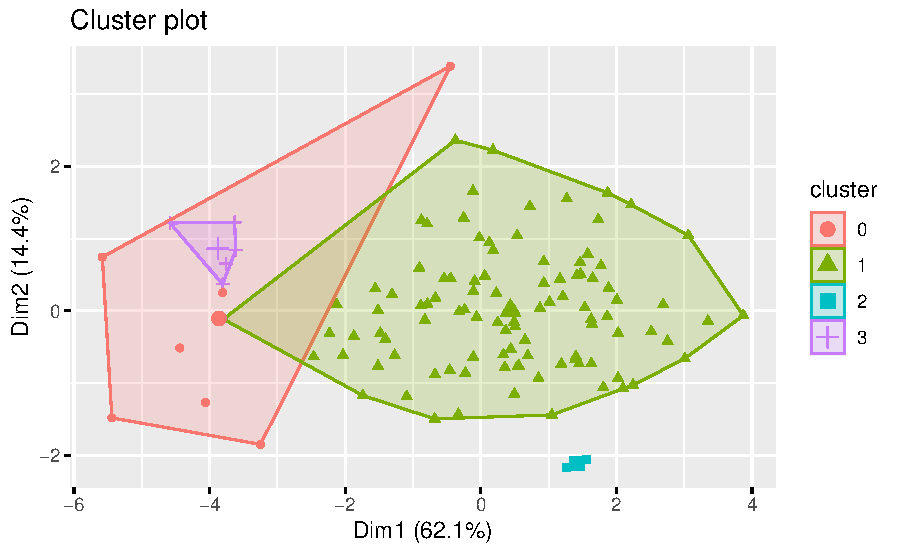
\includegraphics[width=1\linewidth]{figures/unnamed-chunk-17-1} \end{center}

Niestety metoda ta wydaje się niezadowalająca. Znacząca większość obiektów została przypisana do jednego skupienia. Pozostałe 3 skupienia zawierają niewielką liczbę obserwacji.
Biorąc pod uwagę powyższe wyniki grupowania za pomocą różnych metod analizy skupień, zdecydowano w dalszym badaniu wykorzystać wyniki uzyskane za pomocą metody K-średnich.
Podział na 3 skupienia za pomocą analizy skupień pozwolił na określenie trzech poziomów rozwoju (wysoki, średni, niski).

\hypertarget{kla_ad}{%
\section{Klasyfikacja}\label{kla_ad}}

Klasyfikacje metodą lasów losowych wykonano w programie R następującymi instrukcjami wykorzystując funkcję \emph{randomForest}, z pakietu \emph{randomForest} \autocite{R-randomForest}, która tworzy model lasów losowych.

\begin{Shaded}
\begin{Highlighting}[]
\NormalTok{model.forestN }\OtherTok{\textless{}{-}}\NormalTok{ randomForest}\SpecialCharTok{::}\FunctionTok{randomForest}\NormalTok{(}\AttributeTok{formula =}\NormalTok{ Poziom\_Rozwoju }\SpecialCharTok{\textasciitilde{}}
\NormalTok{    ., }\AttributeTok{data =}\NormalTok{ gus2016\_norm, }\AttributeTok{ntree =} \DecValTok{300}\NormalTok{, }\AttributeTok{importance =} \ConstantTok{TRUE}\NormalTok{, }\AttributeTok{proximity =} \ConstantTok{TRUE}\NormalTok{)}
\FunctionTok{plot}\NormalTok{(model.forestN)}
\end{Highlighting}
\end{Shaded}

\begin{center}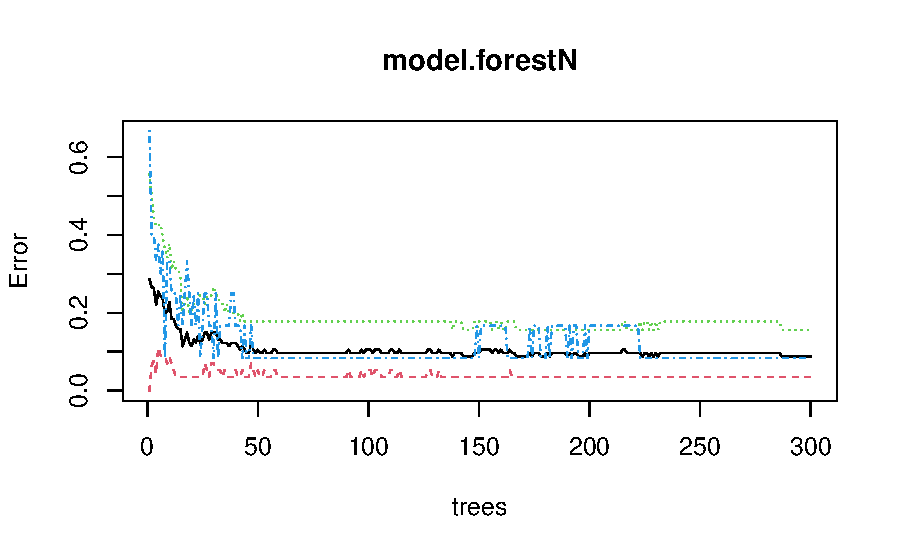
\includegraphics[width=1\linewidth]{figures/unnamed-chunk-18-1} \end{center}

Powyższy wykres przedstawia błąd OOB (ang. \emph{out-of-bag}) - kolor czarny, oraz krzywe wskaźnika błędów błędnej klasyfikacji - kolor niebieski, zielony oraz czerwony. Widać, ze powyżej ok. 150 drzew błąd OOB nie zmniejsza się.

Wykres średniej dokładności spadku (ang. \emph{The Mean Decrease Accuracy}) wyraża, jak dużą dokładność traci model przez wykluczenie każdej zmiennej. Im bardziej ucierpi dokładność, tym ważniejsza jest zmienna dla pomyślnej klasyfikacji. Zmienne są prezentowane według malejącego znaczenia. Średni spadek współczynnika Giniego (ang. \emph{The mean decrease in Gini}) jest miarą tego, jak każda zmienna przyczynia się do jednorodności węzłów i liści w powstałym lesie losowym. Im większa wartość średniej dokładności spadku lub średniego spadku wyniku Giniego, tym większe znaczenie zmiennej w modelu.
Wykres średniej dokładności spadku oraz średniego spadku współczynnika Giniego wykonano następującymi instrukcji za pomocą funkcji \emph{varImpPlot}.

\begin{Shaded}
\begin{Highlighting}[]
\NormalTok{randomForest}\SpecialCharTok{::}\FunctionTok{varImpPlot}\NormalTok{(model.forestN, }\AttributeTok{sort =} \ConstantTok{TRUE}\NormalTok{)}
\end{Highlighting}
\end{Shaded}

\begin{center}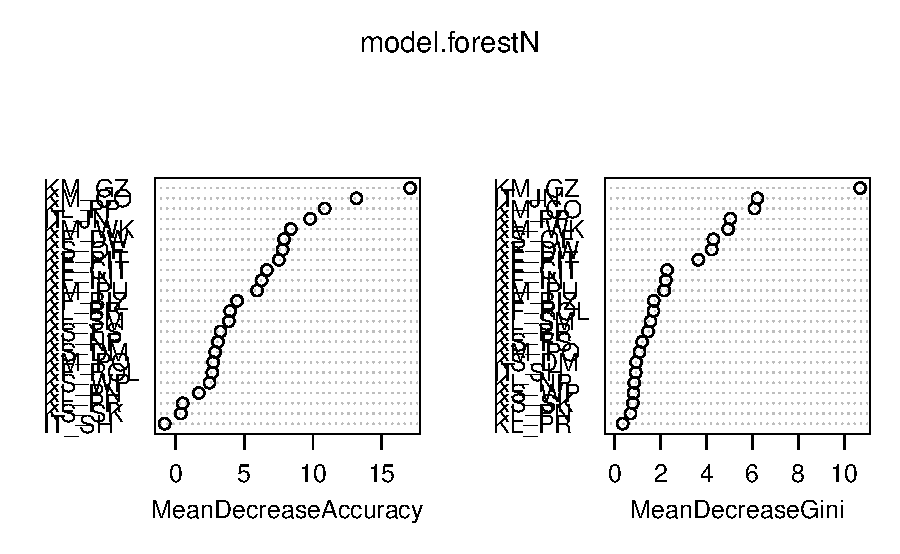
\includegraphics[width=1.05\linewidth]{figures/unnamed-chunk-19-1} \end{center}

Innym narzędziem przedstawiającym istotność czynników stanowiących model lasów losowych jest \emph{plot\_multi\_way\_importance} z pakietu \emph{randomForestExplainer} \autocite{R-randomForestExplainer}

\begin{Shaded}
\begin{Highlighting}[]
\NormalTok{randomForestExplainer}\SpecialCharTok{::}\FunctionTok{plot\_multi\_way\_importance}\NormalTok{(model.forestN,}
    \AttributeTok{no\_of\_labels =} \DecValTok{10}\NormalTok{)}
\end{Highlighting}
\end{Shaded}

\begin{center}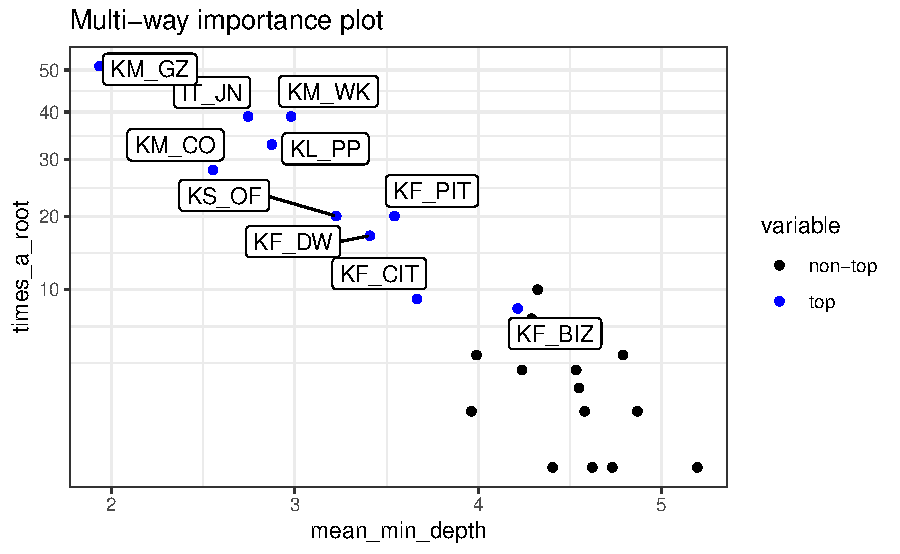
\includegraphics[width=1\linewidth]{figures/unnamed-chunk-20-1} \end{center}

Jak widać wysoki wskaźnik średniej dokładności spadku oraz średnim spadkiem Ginniego charakteryzuje się wskaźnik określający dostępność do gazu (\emph{KM\_GZ} - patrz Tabela \ref{tab:tabela1}), a kolejnym wskaźnikiem jest dostępność do ogrzewania centralnego (\emph{KM\_OG}).
Oba wskaźniki, prócz tej samej kategorii aspektu rozwoju (Kapitał Materialny) są charakterystyczne dla obszarów o zwartej zabudowie.
Model więc w sposób pośredni poinformował nas, że wyższy poziom rozwoju będzie występował na terenach o zwartej zabudowie, czyli uogólniając w miastach.
Następnym istotnym i wiele mówiącym wskaźnikiem są podmioty gospodarcze w sekcjach J-N (\emph{IT\_JN}), czyli uogólniając podmioty dostarczające wysoko wykwalifikowanych usług (finanse, nauka, informatyka).
Co ciekawe drugi wskaźnik z aspektu Innowacji- udział spółek handlowych z udziałem kapitału zagranicznego charakteryzuje się niską istotnością.
Co prowadzi do ciekawych wniosków, jednak może być uwarunkowane lokalną charakterystyką województwa Zachodniopomorskiego.
Wbrew intuicji przyrost naturalny (\emph{KL\_PR}) ma niewielkie znaczenie, prawdopodobnie z~uwagi na jego niewielki rozrzut wśród gmin oraz duże migracje wewnętrzne.
Sugeruje to, że możliwą poprawę modelu uzyska się włączając do modelu przyrost rzeczywisty zamiast przyrostu naturalnego.

Sprawdzono, także istotność syntetycznego wskaźnika poziomu rozwoju społeczno-gospodarczego oraz jego poszczególnych aspektów syntetycznego.

\begin{Shaded}
\begin{Highlighting}[]
\NormalTok{randomForest}\SpecialCharTok{::}\FunctionTok{varImpPlot}\NormalTok{(model.forest, }\AttributeTok{sort =} \ConstantTok{TRUE}\NormalTok{)}
\end{Highlighting}
\end{Shaded}

\begin{center}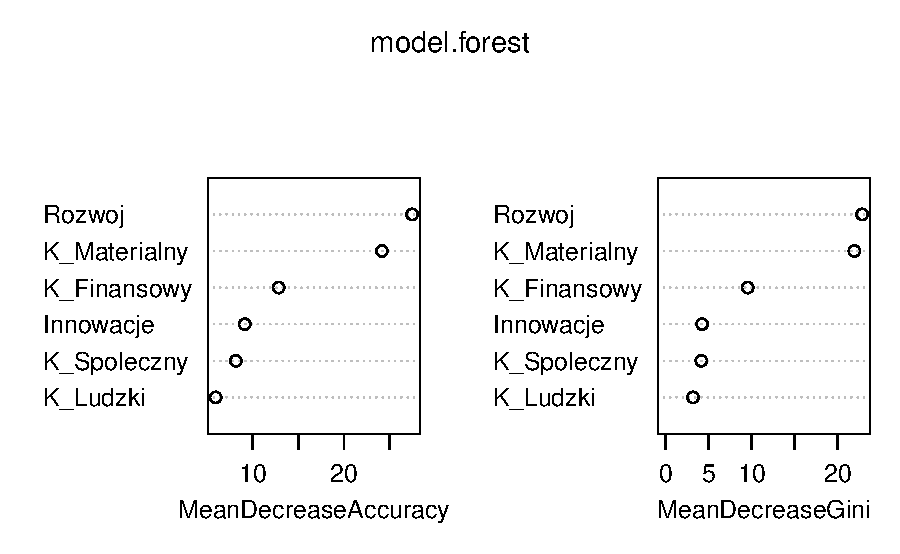
\includegraphics[width=1\linewidth]{figures/unnamed-chunk-22-1} \end{center}

\begin{Shaded}
\begin{Highlighting}[]
\NormalTok{randomForestExplainer}\SpecialCharTok{::}\FunctionTok{plot\_multi\_way\_importance}\NormalTok{(model.forest,}
    \AttributeTok{no\_of\_labels =} \DecValTok{10}\NormalTok{)}
\end{Highlighting}
\end{Shaded}

\begin{center}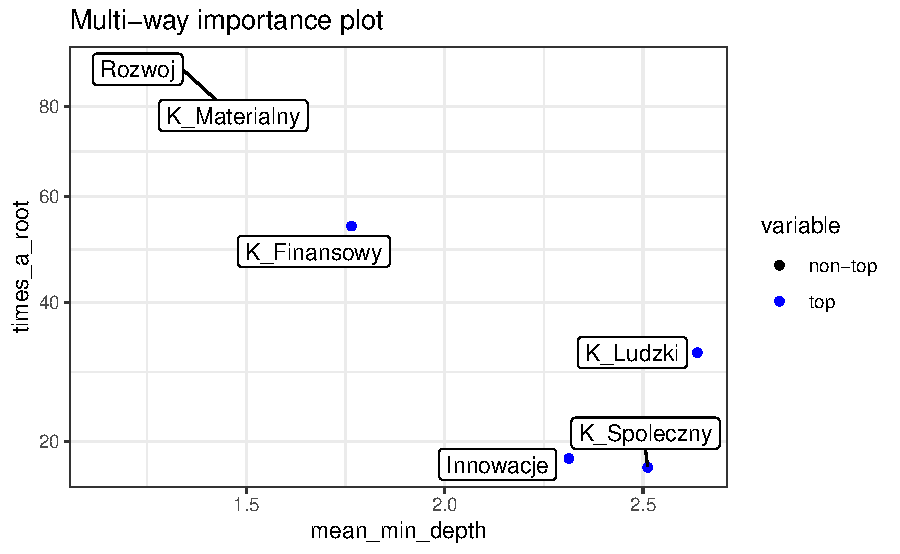
\includegraphics[width=1\linewidth]{figures/unnamed-chunk-23-1} \end{center}

Jak widać najistotniejszymi kategoriami dla modelu jest rozwój społeczno-gospodarczy oraz kapitał materialny.
Istotny jest również kapitał finansowy.
Natomiast Kapitał ludzki, społeczny oraz innowacje cechują się dość niską istotnością.
Na niską istotność innowacji jako aspektu przekłada się niewielka liczba wskaźników innowacji, które brały udział w konstrukcji syntetycznego wskaźnika rozwoju.
Wiemy natomiast, że biorąc pod uwagę wskaźniki, które przekładają się na syntetyczny poziom rozwoju to wskaźnik będący częścią aspektu innowacje miał bardzo duże znaczenie (\emph{IT\_JN}).

Za pomocą poniższych instrukcji korzystając z funkcji \emph{partialPlot} z pakietu \emph{randomForest} wygenerowano wykres częściowej zależności, który daje graficzne przedstawienie wpływu zmiennej na prawdopodobieństwo przydzielenia do danego skupienia.

\begin{Shaded}
\begin{Highlighting}[]
\NormalTok{randomForest}\SpecialCharTok{::}\FunctionTok{partialPlot}\NormalTok{(model.forest, gus2016\_base, Rozwoj,}
    \StringTok{"niski"}\NormalTok{)}
\end{Highlighting}
\end{Shaded}

\begin{center}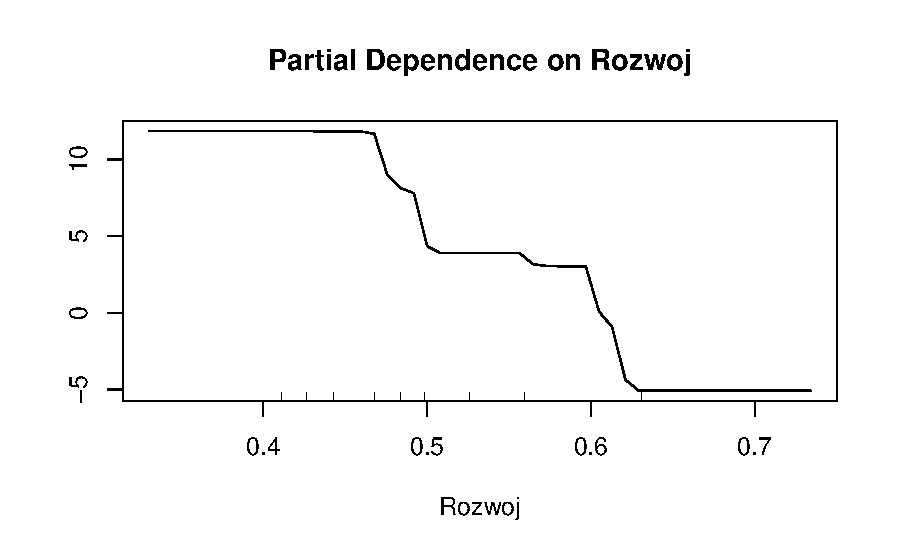
\includegraphics[width=0.9\linewidth]{figures/unnamed-chunk-24-1} \end{center}

Wykres częściowej zależności pokazuje, że gminy o niskim poziomie rozwoju charakteryzują się syntetycznym wskaźnikiem poziomu rozwoju społeczno-gospodarczego na poziomie poniżej \(0.6\), przy czym większość poniżej \(0.45\).

\begin{Shaded}
\begin{Highlighting}[]
\NormalTok{randomForest}\SpecialCharTok{::}\FunctionTok{partialPlot}\NormalTok{(model.forest, gus2016\_base, Rozwoj,}
    \StringTok{"średni"}\NormalTok{)}
\end{Highlighting}
\end{Shaded}

\begin{center}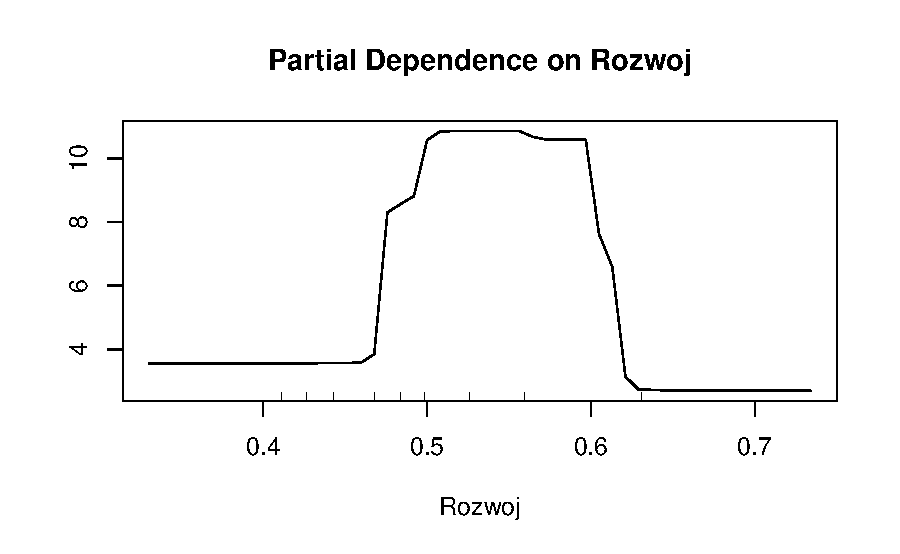
\includegraphics[width=0.9\linewidth]{figures/unnamed-chunk-25-1} \end{center}

Zgodnie z powyższym wykresem, większość gmin (obserwacji) zaklasyfikowanych jako gminy o średnim poziomie rozwoju to gminy, których syntetyczny wskaźnik rozwoju zawiera się w przedziale \(\{0.45,\dots, 0.6\}\)

\begin{Shaded}
\begin{Highlighting}[]
\NormalTok{randomForest}\SpecialCharTok{::}\FunctionTok{partialPlot}\NormalTok{(model.forest, gus2016\_base, Rozwoj,}
    \StringTok{"wysoki"}\NormalTok{)}
\end{Highlighting}
\end{Shaded}

\begin{center}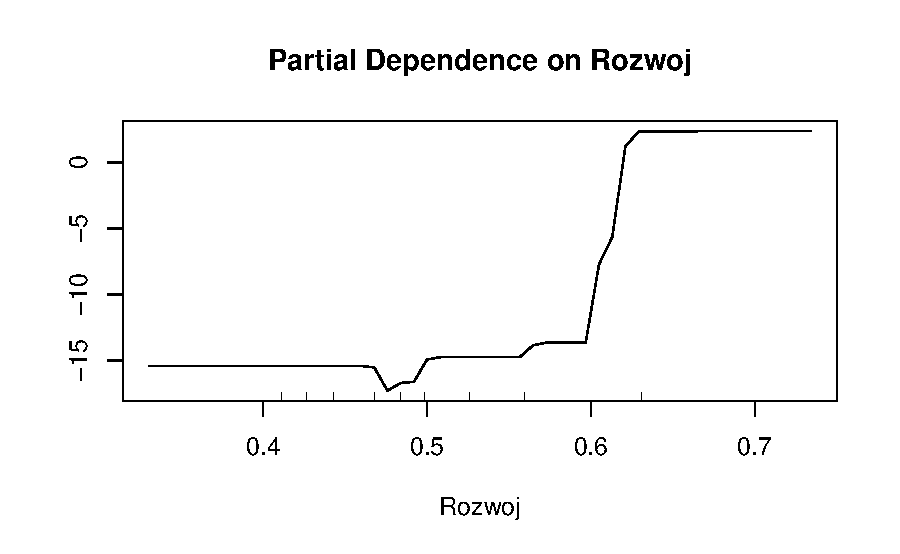
\includegraphics[width=0.9\linewidth]{figures/unnamed-chunk-26-1} \end{center}

Większość gmin zakwalifikowanych jako wysoko rozwinięte charakteryzuje się syntetycznym wskaźnikiem poziomu rozwoju powyżej \(0.6\).

Podobnie przedstawia się wykres pudełkowy ukazujący poziom rozwoju w zależności od syntetycznego wskaźnika poziomu rozwoju społeczno-gospodarczego. Wykres pudełkowy stworzono za pomocą funkcji \emph{ggboxplot} z pakietu \emph{ggpubr} \autocite{R-ggpubr}.

\begin{Shaded}
\begin{Highlighting}[]
\NormalTok{ggpubr}\SpecialCharTok{::}\FunctionTok{ggboxplot}\NormalTok{(gus2016\_base, }\AttributeTok{x =} \StringTok{"Poziom\_Rozwoju"}\NormalTok{, }\AttributeTok{y =} \StringTok{"Rozwoj"}\NormalTok{, }
          \AttributeTok{color =} \StringTok{"Poziom\_Rozwoju"}\NormalTok{,}
          \AttributeTok{xlab =} \StringTok{"Poziom rozwoju"}\NormalTok{, }\AttributeTok{ylab =} \StringTok{"Syntetyczny wskaźnik rozwoju"}\NormalTok{)}
\end{Highlighting}
\end{Shaded}

\begin{center}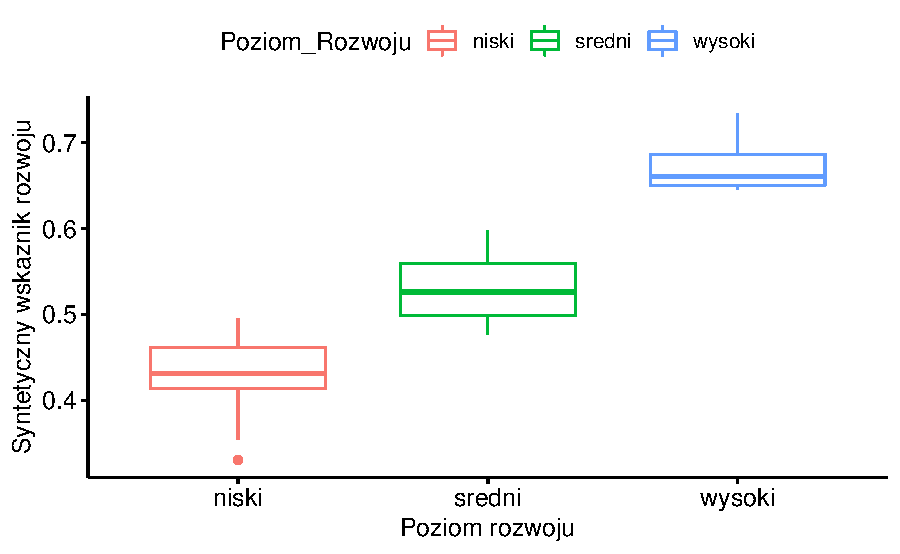
\includegraphics[width=1\linewidth]{figures/unnamed-chunk-27-1} \end{center}

Klasyfikację metodą xgboost wykonano w programie R za pomocą pakietu \emph{xgboost} \autocite{R-xgboost}. Poniższe instrukcje mają na celu stworzenie modelu xgboost.

\begin{Shaded}
\begin{Highlighting}[]
\NormalTok{dtrain }\OtherTok{\textless{}{-}} \FunctionTok{list}\NormalTok{(}\FunctionTok{as.matrix}\NormalTok{(gus2016\_norm[, }\DecValTok{1}\SpecialCharTok{:}\DecValTok{24}\NormalTok{]), }
               \AttributeTok{label =} \FunctionTok{as.numeric}\NormalTok{(gus2016\_norm}\SpecialCharTok{$}\NormalTok{Poziom\_Rozwoju) }\SpecialCharTok{{-}} \DecValTok{1}\NormalTok{)}

\NormalTok{(xgb.fit }\OtherTok{\textless{}{-}}\NormalTok{ xgboost}\SpecialCharTok{::}\FunctionTok{xgboost}\NormalTok{(}\AttributeTok{data =}\NormalTok{ dtrain[[}\DecValTok{1}\NormalTok{]],}
                    \AttributeTok{label =}\NormalTok{ dtrain[[}\DecValTok{2}\NormalTok{]],}
                    \AttributeTok{eta =} \FloatTok{0.1}\NormalTok{, }\CommentTok{\# niższa wartość przeciwdziała przeuczeniu}
                    \AttributeTok{max\_depth =} \DecValTok{10}\NormalTok{, }
                    \AttributeTok{nround =} \DecValTok{100}\NormalTok{, }
                    \AttributeTok{subsample =} \FloatTok{0.5}\NormalTok{, }
                    \AttributeTok{eval\_metric =} \StringTok{\textquotesingle{}mlogloss\textquotesingle{}}\NormalTok{, }
                    \AttributeTok{objective =} \StringTok{\textquotesingle{}multi:softprob\textquotesingle{}}\NormalTok{, }
                    \AttributeTok{num\_class =} \DecValTok{3}\NormalTok{, }
                    \AttributeTok{nthread =} \DecValTok{4}\NormalTok{))}
\CommentTok{\#\textgreater{} [1]  train{-}mlogloss:0.997885 }
\CommentTok{\#\textgreater{} [2]  train{-}mlogloss:0.909257 }
\CommentTok{\#\textgreater{} [3]  train{-}mlogloss:0.838608 }
\CommentTok{\#\textgreater{} [4]  train{-}mlogloss:0.773251 }
\CommentTok{\#\textgreater{} [5]  train{-}mlogloss:0.718040 }
\CommentTok{\#\textgreater{} [6]  train{-}mlogloss:0.668381 }
\CommentTok{\#\textgreater{} [7]  train{-}mlogloss:0.617961 }
\CommentTok{\#\textgreater{} [8]  train{-}mlogloss:0.572172 }
\CommentTok{\#\textgreater{} [9]  train{-}mlogloss:0.530559 }
\CommentTok{\#\textgreater{} [10] train{-}mlogloss:0.494900 }
\CommentTok{\#\textgreater{} [11] train{-}mlogloss:0.460779 }
\CommentTok{\#\textgreater{} [12] train{-}mlogloss:0.430935 }
\CommentTok{\#\textgreater{} [13] train{-}mlogloss:0.404206 }
\CommentTok{\#\textgreater{} [14] train{-}mlogloss:0.380869 }
\CommentTok{\#\textgreater{} [15] train{-}mlogloss:0.356333 }
\CommentTok{\#\textgreater{} [16] train{-}mlogloss:0.336796 }
\CommentTok{\#\textgreater{} [17] train{-}mlogloss:0.318126 }
\CommentTok{\#\textgreater{} [18] train{-}mlogloss:0.298931 }
\CommentTok{\#\textgreater{} [19] train{-}mlogloss:0.282705 }
\CommentTok{\#\textgreater{} [20] train{-}mlogloss:0.266052 }
\CommentTok{\#\textgreater{} [21] train{-}mlogloss:0.253279 }
\CommentTok{\#\textgreater{} [22] train{-}mlogloss:0.240274 }
\CommentTok{\#\textgreater{} [23] train{-}mlogloss:0.229947 }
\CommentTok{\#\textgreater{} [24] train{-}mlogloss:0.218088 }
\CommentTok{\#\textgreater{} [25] train{-}mlogloss:0.209529 }
\CommentTok{\#\textgreater{} [26] train{-}mlogloss:0.199292 }
\CommentTok{\#\textgreater{} [27] train{-}mlogloss:0.189607 }
\CommentTok{\#\textgreater{} [28] train{-}mlogloss:0.181717 }
\CommentTok{\#\textgreater{} [29] train{-}mlogloss:0.173295 }
\CommentTok{\#\textgreater{} [30] train{-}mlogloss:0.166231 }
\CommentTok{\#\textgreater{} [31] train{-}mlogloss:0.159693 }
\CommentTok{\#\textgreater{} [32] train{-}mlogloss:0.153206 }
\CommentTok{\#\textgreater{} [33] train{-}mlogloss:0.147119 }
\CommentTok{\#\textgreater{} [34] train{-}mlogloss:0.141460 }
\CommentTok{\#\textgreater{} [35] train{-}mlogloss:0.136236 }
\CommentTok{\#\textgreater{} [36] train{-}mlogloss:0.132112 }
\CommentTok{\#\textgreater{} [37] train{-}mlogloss:0.127626 }
\CommentTok{\#\textgreater{} [38] train{-}mlogloss:0.123212 }
\CommentTok{\#\textgreater{} [39] train{-}mlogloss:0.118937 }
\CommentTok{\#\textgreater{} [40] train{-}mlogloss:0.114967 }
\CommentTok{\#\textgreater{} [41] train{-}mlogloss:0.111629 }
\CommentTok{\#\textgreater{} [42] train{-}mlogloss:0.107682 }
\CommentTok{\#\textgreater{} [43] train{-}mlogloss:0.104072 }
\CommentTok{\#\textgreater{} [44] train{-}mlogloss:0.100303 }
\CommentTok{\#\textgreater{} [45] train{-}mlogloss:0.097642 }
\CommentTok{\#\textgreater{} [46] train{-}mlogloss:0.095017 }
\CommentTok{\#\textgreater{} [47] train{-}mlogloss:0.092613 }
\CommentTok{\#\textgreater{} [48] train{-}mlogloss:0.089290 }
\CommentTok{\#\textgreater{} [49] train{-}mlogloss:0.087161 }
\CommentTok{\#\textgreater{} [50] train{-}mlogloss:0.084854 }
\CommentTok{\#\textgreater{} [51] train{-}mlogloss:0.082858 }
\CommentTok{\#\textgreater{} [52] train{-}mlogloss:0.080699 }
\CommentTok{\#\textgreater{} [53] train{-}mlogloss:0.078807 }
\CommentTok{\#\textgreater{} [54] train{-}mlogloss:0.077011 }
\CommentTok{\#\textgreater{} [55] train{-}mlogloss:0.075521 }
\CommentTok{\#\textgreater{} [56] train{-}mlogloss:0.073813 }
\CommentTok{\#\textgreater{} [57] train{-}mlogloss:0.072472 }
\CommentTok{\#\textgreater{} [58] train{-}mlogloss:0.070746 }
\CommentTok{\#\textgreater{} [59] train{-}mlogloss:0.069476 }
\CommentTok{\#\textgreater{} [60] train{-}mlogloss:0.068129 }
\CommentTok{\#\textgreater{} [61] train{-}mlogloss:0.067116 }
\CommentTok{\#\textgreater{} [62] train{-}mlogloss:0.065451 }
\CommentTok{\#\textgreater{} [63] train{-}mlogloss:0.063980 }
\CommentTok{\#\textgreater{} [64] train{-}mlogloss:0.062357 }
\CommentTok{\#\textgreater{} [65] train{-}mlogloss:0.060823 }
\CommentTok{\#\textgreater{} [66] train{-}mlogloss:0.059931 }
\CommentTok{\#\textgreater{} [67] train{-}mlogloss:0.059013 }
\CommentTok{\#\textgreater{} [68] train{-}mlogloss:0.058509 }
\CommentTok{\#\textgreater{} [69] train{-}mlogloss:0.057438 }
\CommentTok{\#\textgreater{} [70] train{-}mlogloss:0.056224 }
\CommentTok{\#\textgreater{} [71] train{-}mlogloss:0.055519 }
\CommentTok{\#\textgreater{} [72] train{-}mlogloss:0.054804 }
\CommentTok{\#\textgreater{} [73] train{-}mlogloss:0.054045 }
\CommentTok{\#\textgreater{} [74] train{-}mlogloss:0.053553 }
\CommentTok{\#\textgreater{} [75] train{-}mlogloss:0.052829 }
\CommentTok{\#\textgreater{} [76] train{-}mlogloss:0.052280 }
\CommentTok{\#\textgreater{} [77] train{-}mlogloss:0.051682 }
\CommentTok{\#\textgreater{} [78] train{-}mlogloss:0.050844 }
\CommentTok{\#\textgreater{} [79] train{-}mlogloss:0.050293 }
\CommentTok{\#\textgreater{} [80] train{-}mlogloss:0.049280 }
\CommentTok{\#\textgreater{} [81] train{-}mlogloss:0.049056 }
\CommentTok{\#\textgreater{} [82] train{-}mlogloss:0.048635 }
\CommentTok{\#\textgreater{} [83] train{-}mlogloss:0.048103 }
\CommentTok{\#\textgreater{} [84] train{-}mlogloss:0.047474 }
\CommentTok{\#\textgreater{} [85] train{-}mlogloss:0.047179 }
\CommentTok{\#\textgreater{} [86] train{-}mlogloss:0.046598 }
\CommentTok{\#\textgreater{} [87] train{-}mlogloss:0.046149 }
\CommentTok{\#\textgreater{} [88] train{-}mlogloss:0.045753 }
\CommentTok{\#\textgreater{} [89] train{-}mlogloss:0.045068 }
\CommentTok{\#\textgreater{} [90] train{-}mlogloss:0.044401 }
\CommentTok{\#\textgreater{} [91] train{-}mlogloss:0.043755 }
\CommentTok{\#\textgreater{} [92] train{-}mlogloss:0.043506 }
\CommentTok{\#\textgreater{} [93] train{-}mlogloss:0.042797 }
\CommentTok{\#\textgreater{} [94] train{-}mlogloss:0.042242 }
\CommentTok{\#\textgreater{} [95] train{-}mlogloss:0.042111 }
\CommentTok{\#\textgreater{} [96] train{-}mlogloss:0.041620 }
\CommentTok{\#\textgreater{} [97] train{-}mlogloss:0.041395 }
\CommentTok{\#\textgreater{} [98] train{-}mlogloss:0.041277 }
\CommentTok{\#\textgreater{} [99] train{-}mlogloss:0.041062 }
\CommentTok{\#\textgreater{} [100]    train{-}mlogloss:0.040747}
\CommentTok{\#\textgreater{} \#\#\#\#\# xgb.Booster}
\CommentTok{\#\textgreater{} raw: 207.5 Kb }
\CommentTok{\#\textgreater{} call:}
\CommentTok{\#\textgreater{}   xgb.train(params = params, data = dtrain, nrounds = nrounds, }
\CommentTok{\#\textgreater{}     watchlist = watchlist, verbose = verbose, print\_every\_n = print\_every\_n, }
\CommentTok{\#\textgreater{}     early\_stopping\_rounds = early\_stopping\_rounds, maximize = maximize, }
\CommentTok{\#\textgreater{}     save\_period = save\_period, save\_name = save\_name, xgb\_model = xgb\_model, }
\CommentTok{\#\textgreater{}     callbacks = callbacks, eta = 0.1, max\_depth = 10, subsample = 0.5, }
\CommentTok{\#\textgreater{}     eval\_metric = "mlogloss", objective = "multi:softprob", num\_class = 3, }
\CommentTok{\#\textgreater{}     nthread = 4)}
\CommentTok{\#\textgreater{} params (as set within xgb.train):}
\CommentTok{\#\textgreater{}   eta = "0.1", max\_depth = "10", subsample = "0.5", eval\_metric = "mlogloss", objective = "multi:softprob", num\_class = "3", nthread = "4", validate\_parameters = "TRUE"}
\CommentTok{\#\textgreater{} xgb.attributes:}
\CommentTok{\#\textgreater{}   niter}
\CommentTok{\#\textgreater{} callbacks:}
\CommentTok{\#\textgreater{}   cb.print.evaluation(period = print\_every\_n)}
\CommentTok{\#\textgreater{}   cb.evaluation.log()}
\CommentTok{\#\textgreater{} \# of features: 24 }
\CommentTok{\#\textgreater{} niter: 100}
\CommentTok{\#\textgreater{} nfeatures : 24 }
\CommentTok{\#\textgreater{} evaluation\_log:}
\CommentTok{\#\textgreater{}     iter train\_mlogloss}
\CommentTok{\#\textgreater{}        1       0.997885}
\CommentTok{\#\textgreater{}        2       0.909257}
\CommentTok{\#\textgreater{} {-}{-}{-}                    }
\CommentTok{\#\textgreater{}       99       0.041062}
\CommentTok{\#\textgreater{}      100       0.040747}
\end{Highlighting}
\end{Shaded}

Wykres istotności zmiennych dla modelu xgboost wykonano za pomocą poniższych instrukcji.

\begin{Shaded}
\begin{Highlighting}[]
\NormalTok{xgboost}\SpecialCharTok{::}\FunctionTok{xgb.plot.importance}\NormalTok{(xgboost}\SpecialCharTok{::}\FunctionTok{xgb.importance}\NormalTok{(}\FunctionTok{colnames}\NormalTok{(gus2016\_norm),}
    \AttributeTok{model =}\NormalTok{ xgb.fit))}
\end{Highlighting}
\end{Shaded}

\begin{center}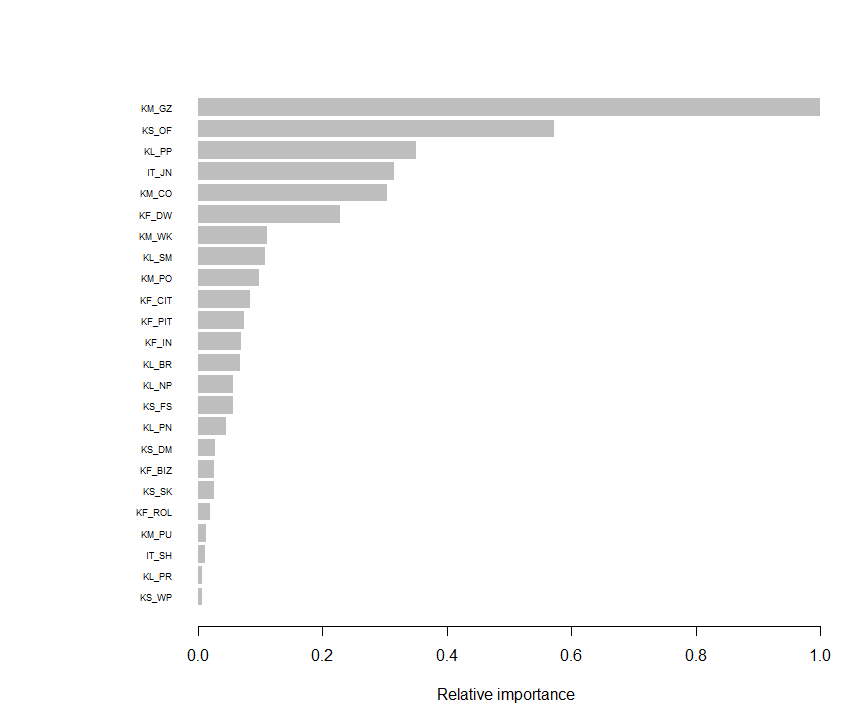
\includegraphics[width=1\linewidth]{figures/xgboost} \end{center}

Zgodnie z powyższym wykresem najistotniejszym czynnikiem jest \emph{KM\_GZ}, czyli podobnie jak przy zastosowaniu przy klasyfikacji metodą lasów losowych.
Kolejnym istotnym czynnikiem jest udział osób fizycznych prowadzących działalność gospodarczą (KS\_OF), wskaźnik ten informuje nas o przedsiębiorczości mieszkańców danej gminy.
Istotny jest też udział osób pracujących w ogóle osób w wieku produkcyjnym oraz dochody własne gminy per capita.
Co ciekawe wskaźnik mający w założeniu przedstawiać jakość rządzenia władzy lokalnej, objawiający się w udziałem specjalistów, kierowników w ogóle radnych nie ma istotnego znaczenia na poziom rozwoju.
Niezwykle istotną role zwartej tkanki przestrzennej na poziom rozwoju społeczno-gospodarczego potwierdza, oprócz wskaźników \emph{KM\_GZ}, \emph{KM\_CO} niska istotność dochodów z podatku rolnego na mieszkańca (\emph{KF\_ROL}).

Za pomocą poniższych instrukcji za pomocą funkcji \emph{xgb.plot.multi.trees} można przedstawić zespół drzew decyzyjnych jako zbiorczą jednostkę.

\begin{Shaded}
\begin{Highlighting}[]
\NormalTok{xgboost}\SpecialCharTok{::}\FunctionTok{xgb.plot.multi.trees}\NormalTok{(}\FunctionTok{colnames}\NormalTok{(gus2016\_norm), }\AttributeTok{model =}\NormalTok{ xgb.fit)}
\CommentTok{\#\textgreater{} Column 2 [\textquotesingle{}No\textquotesingle{}] of item 2 is missing in item 1. Use fill=TRUE to fill with NA (NULL for list columns), or use.names=FALSE to ignore column names. use.names=\textquotesingle{}check\textquotesingle{} (default from v1.12.2) emits this message and proceeds as if use.names=FALSE for  backwards compatibility. See news item 5 in v1.12.2 for options to control this message.}
\end{Highlighting}
\end{Shaded}

\textbackslash begin\{center\}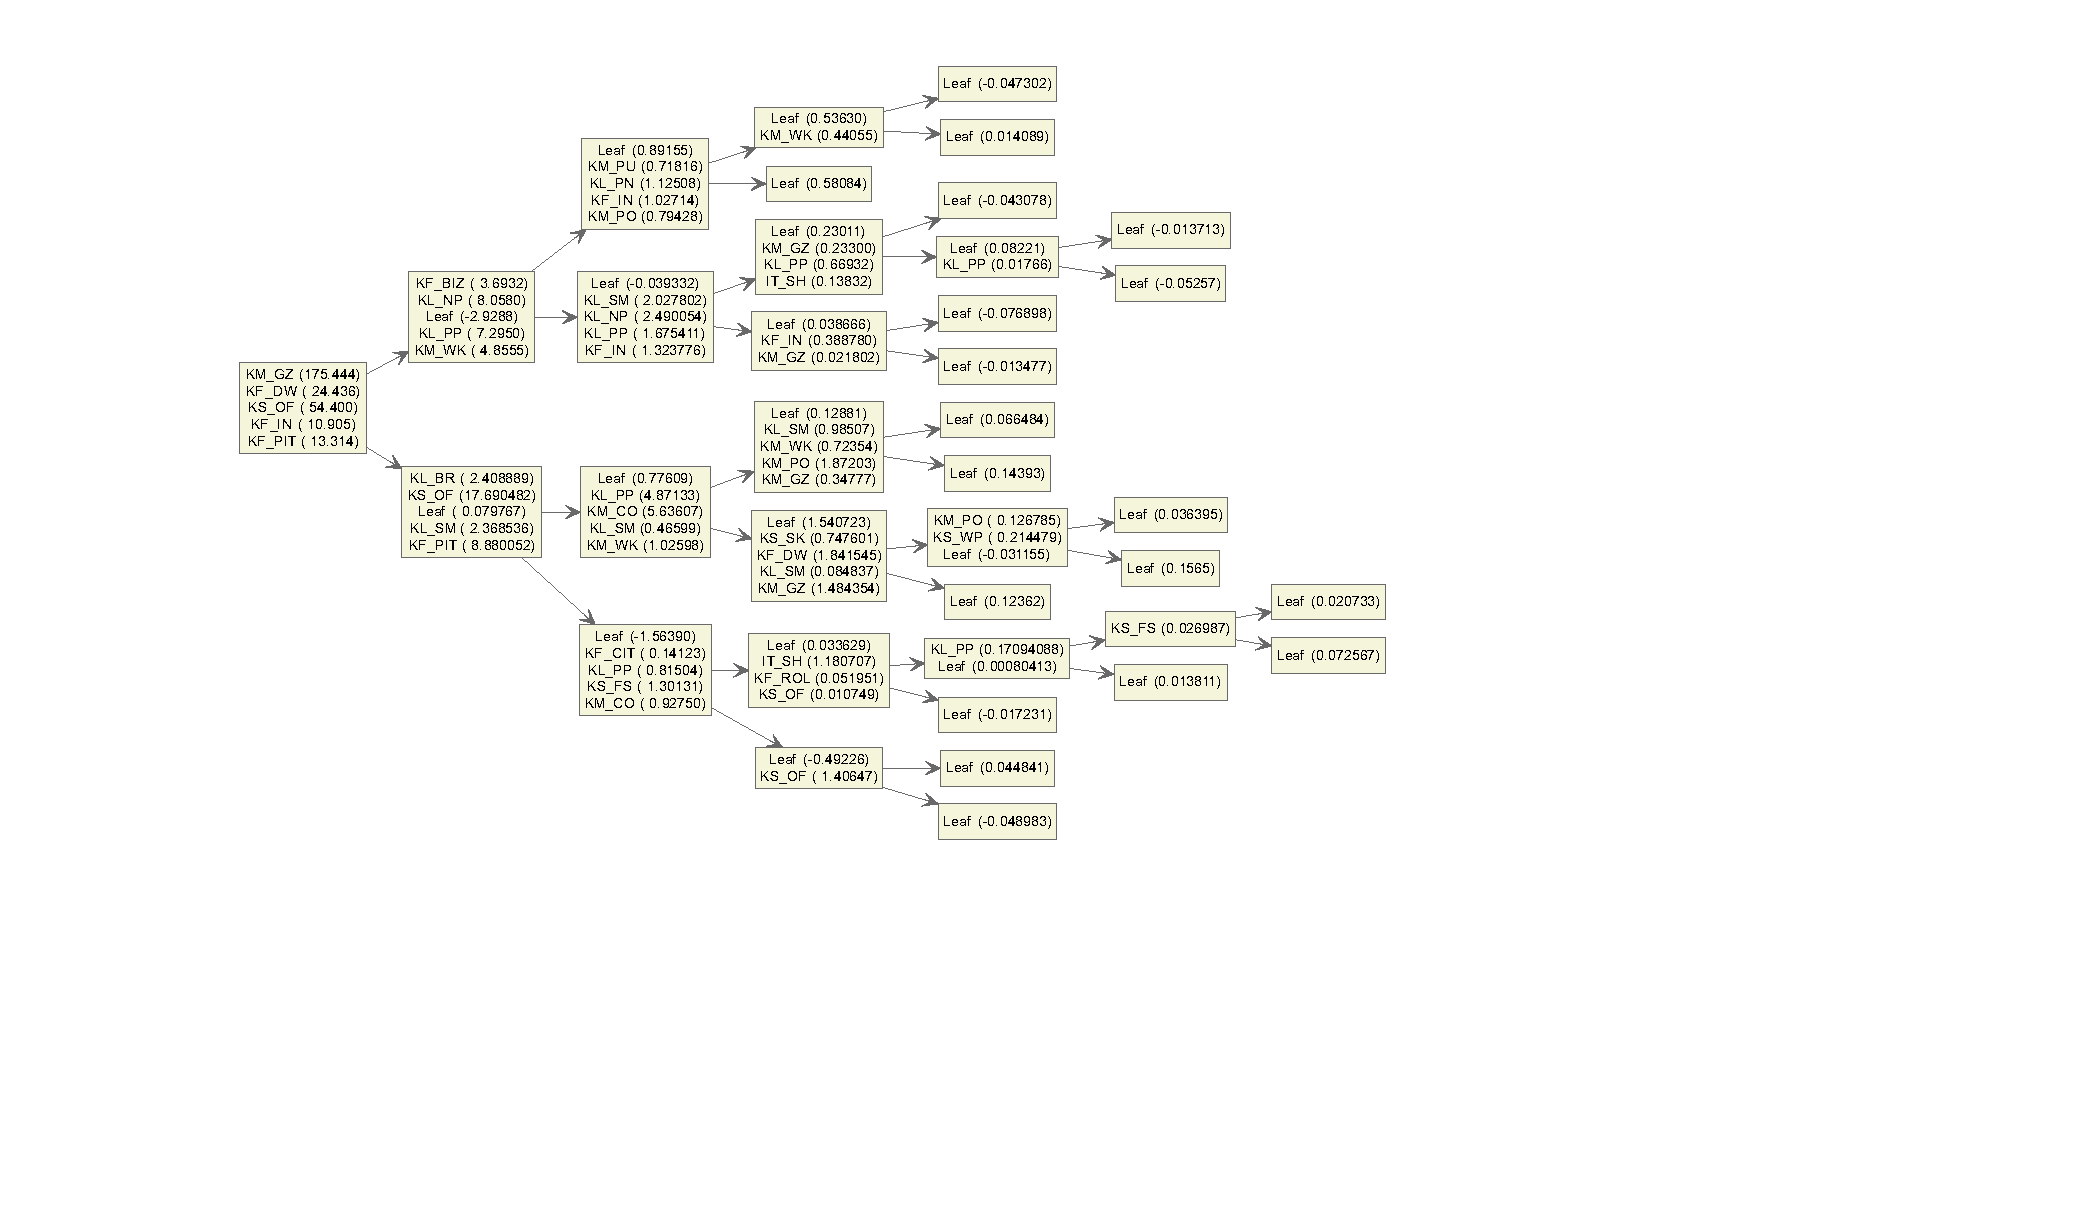
\includegraphics[width=1\linewidth]{figures/unnamed-chunk-30-1}

\hypertarget{aw_ad}{%
\section{Analiza wariancji}\label{aw_ad}}

Jednoczynnikową analizę wariancji (ang. \emph{one-way ANOVA}) wykonujemy w programie R następującymi instrukcjami wykorzystując funkcję \emph{aov} z pakietu \emph{stats} \autocite{R-stats}. Funkcja \emph{summary} służy do podsumowania modelu analizy wariancji.

\begin{Shaded}
\begin{Highlighting}[]
\CommentTok{\# ANOVA}
\NormalTok{ANOVA }\OtherTok{\textless{}{-}}\NormalTok{ stats}\SpecialCharTok{::}\FunctionTok{aov}\NormalTok{(gus2016\_base}\SpecialCharTok{$}\NormalTok{Rozwoj }\SpecialCharTok{\textasciitilde{}}\NormalTok{ gus2016\_base}\SpecialCharTok{$}\NormalTok{Poziom\_Rozwoju)}
\FunctionTok{summary}\NormalTok{(ANOVA)}
\CommentTok{\#\textgreater{}                              Df Sum Sq Mean Sq F value Pr(\textgreater{}F)    }
\CommentTok{\#\textgreater{} gus2016\_base$Poziom\_Rozwoju   2 0.6485  0.3242     269 \textless{}2e{-}16 ***}
\CommentTok{\#\textgreater{} Residuals                   111 0.1338  0.0012                   }
\CommentTok{\#\textgreater{} {-}{-}{-}}
\CommentTok{\#\textgreater{} Signif. codes:  0 \textquotesingle{}***\textquotesingle{} 0.001 \textquotesingle{}**\textquotesingle{} 0.01 \textquotesingle{}*\textquotesingle{} 0.05 \textquotesingle{}.\textquotesingle{} 0.1 \textquotesingle{} \textquotesingle{} 1}
\end{Highlighting}
\end{Shaded}

Ponieważ \(p\)-wartość jest mniejsza niż poziom istotności \(0.001\) to mamy podstawy, żeby odrzucić hipotezę zerową.
Średnie grupowe różnią się znacząco między sobą.
Możemy stwierdzić, że poziom rozwoju ma istotny wpływ na syntetyczny wskaźnik poziomu rozwoju społeczno-gospodarczego oraz jego aspekty (oznaczone jako reszty z~modelu - ang. \emph{Residuals})

W jednoczynnikowej analizie wariancji istotna \(p\)-wartość wskazuje, że niektóre średnie grupowe są różne, ale nie wiemy, które pary grup są różne.
Możliwe jest przeprowadzenie wielokrotnych porównań parami, aby określić, czy średnia różnica między poszczególnymi parami grupy jest statystycznie istotna.

W tym celu wykonano test Tukey-a (jeden z testów post hoc) za pomocą funkcji \emph{TukeyHSD} z pakietu \emph{stats}

\begin{Shaded}
\begin{Highlighting}[]
\CommentTok{\# testy post{-}hoc}
\FunctionTok{TukeyHSD}\NormalTok{(ANOVA)}
\CommentTok{\#\textgreater{}   Tukey multiple comparisons of means}
\CommentTok{\#\textgreater{}     95\% family{-}wise confidence level}
\CommentTok{\#\textgreater{} }
\CommentTok{\#\textgreater{} Fit: stats::aov(formula = gus2016\_base$Rozwoj \textasciitilde{} gus2016\_base$Poziom\_Rozwoju)}
\CommentTok{\#\textgreater{} }
\CommentTok{\#\textgreater{} $\textasciigrave{}gus2016\_base$Poziom\_Rozwoju\textasciigrave{}}
\CommentTok{\#\textgreater{}                     diff        lwr       upr p adj}
\CommentTok{\#\textgreater{} średni{-}niski  0.09563711 0.07919022 0.1120840     0}
\CommentTok{\#\textgreater{} wysoki{-}niski  0.23961273 0.21341741 0.2658080     0}
\CommentTok{\#\textgreater{} wysoki{-}średni 0.14397562 0.11717976 0.1707715     0}
\end{Highlighting}
\end{Shaded}

Zgodnie z powyższym wszystkie pary istotnie się różnią, ponieważ \(p\)-wartość dla każdej z pary wynosi \(0\).
Przy czym największa różnica w średnich jest między poziomami wysoki-niski, co świadczy dobrze o podziale. Różnica między wysokim a średnim poziomem jest większa niż między średnim a niskim.
Może to świadczyć o postępującej polaryzacji rozwoju, żeby to sprawdzić przeprowadzono testy ANOVA i post-hoc Tukeya dla innych roczników.

\begin{Shaded}
\begin{Highlighting}[]
\CommentTok{\# testy post{-}hoc}
\NormalTok{ANOVA }\OtherTok{\textless{}{-}}\NormalTok{ stats}\SpecialCharTok{::}\FunctionTok{aov}\NormalTok{(gus2017\_base}\SpecialCharTok{$}\NormalTok{Rozwoj }\SpecialCharTok{\textasciitilde{}}\NormalTok{ gus2017\_base}\SpecialCharTok{$}\NormalTok{Poziom\_Rozwoju)}
\FunctionTok{summary}\NormalTok{(ANOVA)}
\CommentTok{\#\textgreater{}                              Df Sum Sq Mean Sq F value Pr(\textgreater{}F)    }
\CommentTok{\#\textgreater{} gus2017\_base$Poziom\_Rozwoju   2 0.6119 0.30597   253.8 \textless{}2e{-}16 ***}
\CommentTok{\#\textgreater{} Residuals                   111 0.1338 0.00121                   }
\CommentTok{\#\textgreater{} {-}{-}{-}}
\CommentTok{\#\textgreater{} Signif. codes:  0 \textquotesingle{}***\textquotesingle{} 0.001 \textquotesingle{}**\textquotesingle{} 0.01 \textquotesingle{}*\textquotesingle{} 0.05 \textquotesingle{}.\textquotesingle{} 0.1 \textquotesingle{} \textquotesingle{} 1}
\FunctionTok{TukeyHSD}\NormalTok{(ANOVA)}
\CommentTok{\#\textgreater{}   Tukey multiple comparisons of means}
\CommentTok{\#\textgreater{}     95\% family{-}wise confidence level}
\CommentTok{\#\textgreater{} }
\CommentTok{\#\textgreater{} Fit: stats::aov(formula = gus2017\_base$Rozwoj \textasciitilde{} gus2017\_base$Poziom\_Rozwoju)}
\CommentTok{\#\textgreater{} }
\CommentTok{\#\textgreater{} $\textasciigrave{}gus2017\_base$Poziom\_Rozwoju\textasciigrave{}}
\CommentTok{\#\textgreater{}                     diff        lwr       upr p adj}
\CommentTok{\#\textgreater{} średni{-}niski  0.08358656 0.06686513 0.1003080     0}
\CommentTok{\#\textgreater{} wysoki{-}niski  0.21762703 0.19409653 0.2411575     0}
\CommentTok{\#\textgreater{} wysoki{-}średni 0.13404047 0.11002986 0.1580511     0}
\end{Highlighting}
\end{Shaded}

\begin{Shaded}
\begin{Highlighting}[]
\CommentTok{\# testy post{-}hoc}
\NormalTok{ANOVA }\OtherTok{\textless{}{-}}\NormalTok{ stats}\SpecialCharTok{::}\FunctionTok{aov}\NormalTok{(gus2018\_base}\SpecialCharTok{$}\NormalTok{Rozwoj }\SpecialCharTok{\textasciitilde{}}\NormalTok{ gus2018\_base}\SpecialCharTok{$}\NormalTok{Poziom\_Rozwoju)}
\FunctionTok{summary}\NormalTok{(ANOVA)}
\CommentTok{\#\textgreater{}                              Df Sum Sq Mean Sq F value Pr(\textgreater{}F)    }
\CommentTok{\#\textgreater{} gus2018\_base$Poziom\_Rozwoju   2 0.6045 0.30227   285.4 \textless{}2e{-}16 ***}
\CommentTok{\#\textgreater{} Residuals                   111 0.1175 0.00106                   }
\CommentTok{\#\textgreater{} {-}{-}{-}}
\CommentTok{\#\textgreater{} Signif. codes:  0 \textquotesingle{}***\textquotesingle{} 0.001 \textquotesingle{}**\textquotesingle{} 0.01 \textquotesingle{}*\textquotesingle{} 0.05 \textquotesingle{}.\textquotesingle{} 0.1 \textquotesingle{} \textquotesingle{} 1}
\FunctionTok{TukeyHSD}\NormalTok{(ANOVA)}
\CommentTok{\#\textgreater{}   Tukey multiple comparisons of means}
\CommentTok{\#\textgreater{}     95\% family{-}wise confidence level}
\CommentTok{\#\textgreater{} }
\CommentTok{\#\textgreater{} Fit: stats::aov(formula = gus2018\_base$Rozwoj \textasciitilde{} gus2018\_base$Poziom\_Rozwoju)}
\CommentTok{\#\textgreater{} }
\CommentTok{\#\textgreater{} $\textasciigrave{}gus2018\_base$Poziom\_Rozwoju\textasciigrave{}}
\CommentTok{\#\textgreater{}                     diff        lwr       upr p adj}
\CommentTok{\#\textgreater{} średni{-}niski  0.09075572 0.07527941 0.1062320     0}
\CommentTok{\#\textgreater{} wysoki{-}niski  0.22656744 0.20276805 0.2503668     0}
\CommentTok{\#\textgreater{} wysoki{-}średni 0.13581172 0.11147047 0.1601530     0}
\end{Highlighting}
\end{Shaded}

\begin{Shaded}
\begin{Highlighting}[]
\CommentTok{\# testy post{-}hoc}
\NormalTok{ANOVA }\OtherTok{\textless{}{-}}\NormalTok{ stats}\SpecialCharTok{::}\FunctionTok{aov}\NormalTok{(gus2019\_base}\SpecialCharTok{$}\NormalTok{Rozwoj }\SpecialCharTok{\textasciitilde{}}\NormalTok{ gus2019\_base}\SpecialCharTok{$}\NormalTok{Poziom\_Rozwoju)}
\FunctionTok{summary}\NormalTok{(ANOVA)}
\CommentTok{\#\textgreater{}                              Df Sum Sq Mean Sq F value Pr(\textgreater{}F)    }
\CommentTok{\#\textgreater{} gus2019\_base$Poziom\_Rozwoju   2 0.6541  0.3270     275 \textless{}2e{-}16 ***}
\CommentTok{\#\textgreater{} Residuals                   110 0.1308  0.0012                   }
\CommentTok{\#\textgreater{} {-}{-}{-}}
\CommentTok{\#\textgreater{} Signif. codes:  0 \textquotesingle{}***\textquotesingle{} 0.001 \textquotesingle{}**\textquotesingle{} 0.01 \textquotesingle{}*\textquotesingle{} 0.05 \textquotesingle{}.\textquotesingle{} 0.1 \textquotesingle{} \textquotesingle{} 1}
\FunctionTok{TukeyHSD}\NormalTok{(ANOVA)}
\CommentTok{\#\textgreater{}   Tukey multiple comparisons of means}
\CommentTok{\#\textgreater{}     95\% family{-}wise confidence level}
\CommentTok{\#\textgreater{} }
\CommentTok{\#\textgreater{} Fit: stats::aov(formula = gus2019\_base$Rozwoj \textasciitilde{} gus2019\_base$Poziom\_Rozwoju)}
\CommentTok{\#\textgreater{} }
\CommentTok{\#\textgreater{} $\textasciigrave{}gus2019\_base$Poziom\_Rozwoju\textasciigrave{}}
\CommentTok{\#\textgreater{}                     diff        lwr       upr p adj}
\CommentTok{\#\textgreater{} średni{-}niski  0.09599066 0.07960284 0.1123785     0}
\CommentTok{\#\textgreater{} wysoki{-}niski  0.23991372 0.21440405 0.2654234     0}
\CommentTok{\#\textgreater{} wysoki{-}średni 0.14392306 0.11841339 0.1694327     0}
\end{Highlighting}
\end{Shaded}

Powyższe testy prowadzą do ciekawych wniosków.
W 2017 roku znacząco zmniejszyła się polaryzacja poziomu rozwoju w województwie Zachodniopomorskim.
Następnie sukcesywnie co roku wzrastała i w 2019 roku osiągnęła wyższy poziom niż w 2016 roku.
Można również użyć jednoczesnych testów ogólnych hipotez liniowych wielokrotnego porównywania średnich metodą Tukey-a za pomocą pakietu \emph{multcomp} \autocite{R-multcomp}

\begin{Shaded}
\begin{Highlighting}[]
\FunctionTok{summary}\NormalTok{(multcomp}\SpecialCharTok{::}\FunctionTok{glht}\NormalTok{(ANOVA, }\AttributeTok{lincft =} \FunctionTok{mcp}\NormalTok{(}\AttributeTok{group =} \StringTok{"Tukey"}\NormalTok{)))}
\CommentTok{\#\textgreater{} }
\CommentTok{\#\textgreater{}   Simultaneous Tests for General Linear Hypotheses}
\CommentTok{\#\textgreater{} }
\CommentTok{\#\textgreater{} Fit: stats::aov(formula = gus2019\_base$Rozwoj \textasciitilde{} gus2019\_base$Poziom\_Rozwoju)}
\CommentTok{\#\textgreater{} }
\CommentTok{\#\textgreater{} Linear Hypotheses:}
\CommentTok{\#\textgreater{}                                        Estimate Std. Error t value Pr(\textgreater{}|t|)    }
\CommentTok{\#\textgreater{} (Intercept) == 0                       0.430581   0.004877   88.28   \textless{}2e{-}16 ***}
\CommentTok{\#\textgreater{} gus2019\_base$Poziom\_Rozwojuśredni == 0 0.095991   0.006898   13.92   \textless{}2e{-}16 ***}
\CommentTok{\#\textgreater{} gus2019\_base$Poziom\_Rozwojuwysoki == 0 0.239914   0.010737   22.34   \textless{}2e{-}16 ***}
\CommentTok{\#\textgreater{} {-}{-}{-}}
\CommentTok{\#\textgreater{} Signif. codes:  0 \textquotesingle{}***\textquotesingle{} 0.001 \textquotesingle{}**\textquotesingle{} 0.01 \textquotesingle{}*\textquotesingle{} 0.05 \textquotesingle{}.\textquotesingle{} 0.1 \textquotesingle{} \textquotesingle{} 1}
\CommentTok{\#\textgreater{} (Adjusted p values reported {-}{-} single{-}step method)}
\end{Highlighting}
\end{Shaded}

Także ten test odrzucił hipotezę zerową, \(p\)-wartość dla każdego przypadku jest mniejsza niż \(0.001\)

Ponieważ ANOVA zakłada, że dane mają rozkład normalny, a wariancja między grupami jest jednorodna to należy to sprawdzić.
Jednorodność wariancji między grupami sprawdzono dzięki wykresowi reszt w funkcji dopasowań za pomocą następującej instrukcji.

\begin{Shaded}
\begin{Highlighting}[]
\FunctionTok{plot}\NormalTok{(ANOVA, }\DecValTok{1}\NormalTok{)}
\end{Highlighting}
\end{Shaded}

\begin{center}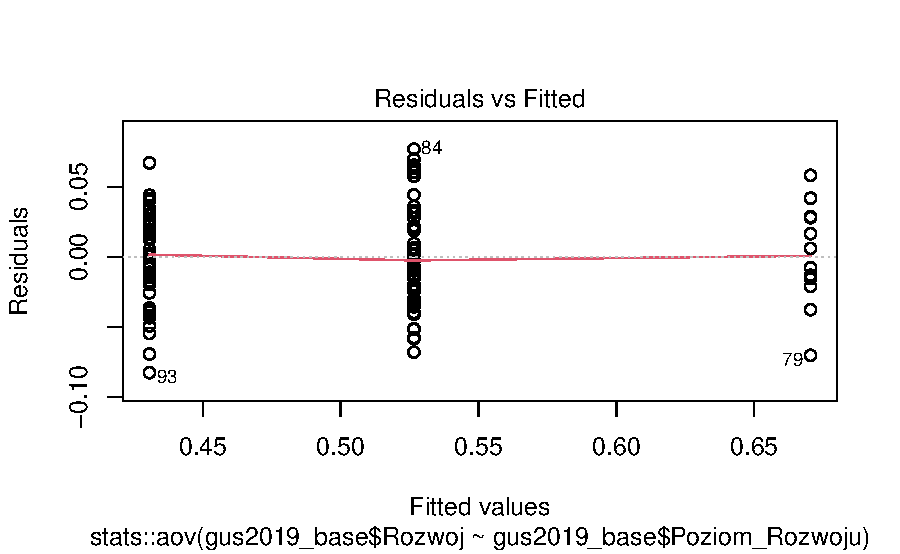
\includegraphics[width=1\linewidth]{figures/unnamed-chunk-37-1} \end{center}

Zgodnie z~powyższym wykresem nie ma ewidentnych zależności między resztami a~średnią z każdej grupy.
Można więc założyć jednorodność wariancji.

Innym sposobem na sprawdzenie jednorodności wariancji jest test Levene, który można wykonać za pomocą funkcji \emph{leveneTest} z pakietu \emph{car} \autocite{R-car}.

\begin{Shaded}
\begin{Highlighting}[]
\NormalTok{car}\SpecialCharTok{::}\FunctionTok{leveneTest}\NormalTok{(gus2016\_base}\SpecialCharTok{$}\NormalTok{Rozwoj }\SpecialCharTok{\textasciitilde{}}\NormalTok{ gus2016\_base}\SpecialCharTok{$}\NormalTok{Poziom\_Rozwoju)}
\CommentTok{\#\textgreater{} Levene\textquotesingle{}s Test for Homogeneity of Variance (center = median)}
\CommentTok{\#\textgreater{}        Df F value Pr(\textgreater{}F)}
\CommentTok{\#\textgreater{} group   2  0.4087 0.6655}
\CommentTok{\#\textgreater{}       111}
\end{Highlighting}
\end{Shaded}

\(p\)-wartość tego testu jest większa niż poziom istotności \(0,05\). Oznacza to, że nie ma dowodów sugerujących, że wariancja między grupami jest istotnie różna. Można założyć jednorodność wariancji w różnych grupach.

Normalność rozkładu można sprawdzić za pomocą wykresu normalności reszt (wykres kwantyl-kwantyl zastosowany do reszt), za pomocą poniższej instrukcji.

\begin{Shaded}
\begin{Highlighting}[]
\FunctionTok{plot}\NormalTok{(ANOVA, }\DecValTok{2}\NormalTok{)}
\end{Highlighting}
\end{Shaded}

\begin{center}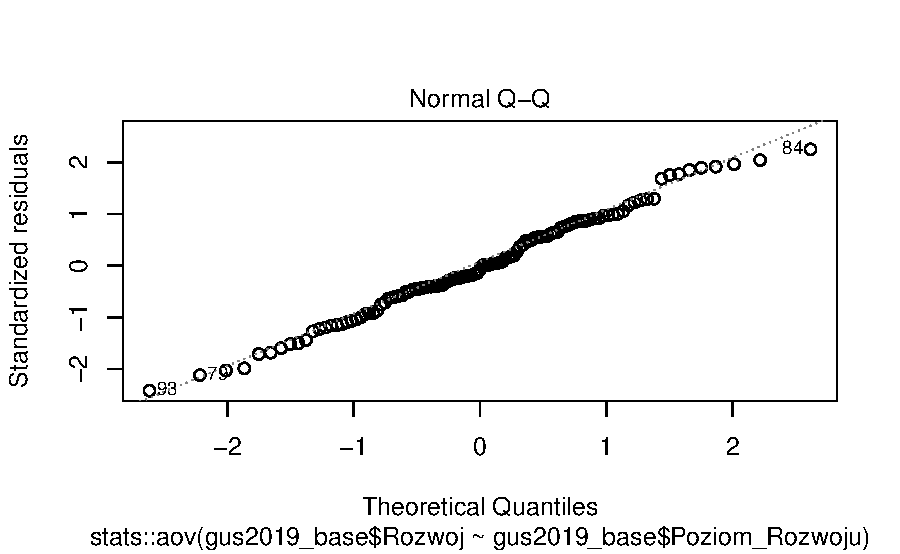
\includegraphics[width=1\linewidth]{figures/unnamed-chunk-39-1} \end{center}

Reszty w przybliżeniu przebiegają wzdłuż linii prostej (45\(^\circ\) linii odniesienia), co sugeruje, że można założyć normalność danych.

Powyższe założenie można potwierdzić stosując test Shapiro-Wilka na resztach ANOVA za pomocą poniższych instrukcji, wykorzystując funkcje \emph{shapiro.test} z pakietu \emph{stats}. Test ten nie wykazuje żadnych oznak naruszenia normalności.

\begin{Shaded}
\begin{Highlighting}[]
\CommentTok{\# test shapiro{-}wilka na resztach w celu sprawdzenia}
\CommentTok{\# normalności}
\NormalTok{ANOVA\_reszty }\OtherTok{\textless{}{-}} \FunctionTok{residuals}\NormalTok{(}\AttributeTok{object =}\NormalTok{ ANOVA)}
\NormalTok{stats}\SpecialCharTok{::}\FunctionTok{shapiro.test}\NormalTok{(}\AttributeTok{x =}\NormalTok{ ANOVA\_reszty)}
\CommentTok{\#\textgreater{} }
\CommentTok{\#\textgreater{}  Shapiro{-}Wilk normality test}
\CommentTok{\#\textgreater{} }
\CommentTok{\#\textgreater{} data:  ANOVA\_reszty}
\CommentTok{\#\textgreater{} W = 0.99041, p{-}value = 0.6155}
\end{Highlighting}
\end{Shaded}

Zgodnie z powyższym \(p\)-wartość jest większa niż \(0.05\) można więc założyć normalność danych.
Potwierdzono, że dane mają rozkład normalny, a wariancja między grupami jest jednorodna.

Wykonano także nieparametryczny test sumy rang Kruskala-Wallisa, który nie wymaga założenia normalności oraz jednorodności wariancji między grupami.
Test Kruskala-Wallisa wykonano za pomocą funkcji \emph{kruskal.test} z pakietu \emph{stats}:

\begin{Shaded}
\begin{Highlighting}[]
\CommentTok{\# test Kruskala{-}Wallis}
\NormalTok{stats}\SpecialCharTok{::}\FunctionTok{kruskal.test}\NormalTok{(gus2016\_base}\SpecialCharTok{$}\NormalTok{Rozwoj }\SpecialCharTok{\textasciitilde{}}\NormalTok{ gus2016\_base}\SpecialCharTok{$}\NormalTok{Poziom\_Rozwoju)}
\CommentTok{\#\textgreater{} }
\CommentTok{\#\textgreater{}  Kruskal{-}Wallis rank sum test}
\CommentTok{\#\textgreater{} }
\CommentTok{\#\textgreater{} data:  gus2016\_base$Rozwoj by gus2016\_base$Poziom\_Rozwoju}
\CommentTok{\#\textgreater{} Kruskal{-}Wallis chi{-}squared = 88.85, df = 2, p{-}value \textless{} 2.2e{-}16}
\end{Highlighting}
\end{Shaded}

Zgodnie z powyższym przyjmujemy hipotezę alternatywną informującą nas o tym, że nie wszystkie mediany grupy są równe. Potwierdza to wnioski płynące z testu ANOVA, dlatego też nie wykonano testów post-hoc dla testu sumy rang Kruskala-Wallisa.

\hypertarget{mapy}{%
\section{Wyniki dla ostatecznych grup -mapy}\label{mapy}}

W celu przedstawienia syntetycznego wskaźnika poziomu rozwoju społeczno-gospodarczego należało przygotować mapy, ukazujące rozmieszczenie przestrzenne rozwoju.
W tym celu skorzystano z danych (plik w formacie \emph{shapefile} - \emph{shp}) dotyczących granic administracyjnych (gmin) z Głównego Urzędu Geodezji i Kartografii.
Dane te obejmowały całą Polskę, dlatego korzystając z programu QGIS ograniczono je do województwa Zachodniopomorskiego.
Następnie za pomocą biblioteki \emph{sf} wczytano przygotowany plik \emph{shp} do środowiska R za pomocą funkcji \emph{read\_sf}:

\begin{Shaded}
\begin{Highlighting}[]
\NormalTok{gminy2 }\OtherTok{\textless{}{-}}\NormalTok{ sf}\SpecialCharTok{::}\FunctionTok{read\_sf}\NormalTok{(}\StringTok{\textquotesingle{}zachpom\_gminy.shp\textquotesingle{}}\NormalTok{)}
\end{Highlighting}
\end{Shaded}

Następnie przygotowano dane dotyczące poziomu rozwoju oraz jego aspektów tak, żeby połączyć je z mapą. Zrobiono to za pomocą poniższych instrukcji.

\begin{Shaded}
\begin{Highlighting}[]
\NormalTok{data\_map2016 }\OtherTok{\textless{}{-}} \FunctionTok{select}\NormalTok{(Gus\_2016, }\DecValTok{1}\SpecialCharTok{:}\DecValTok{2}\NormalTok{)}
\NormalTok{data\_map2016}\SpecialCharTok{$}\NormalTok{ID }\OtherTok{\textless{}{-}} \FunctionTok{seq.int}\NormalTok{(}\FunctionTok{nrow}\NormalTok{(data\_map2016))  }\CommentTok{\#dodaje ID}

\NormalTok{data\_map2016\_temp }\OtherTok{\textless{}{-}}\NormalTok{ dplyr}\SpecialCharTok{::}\FunctionTok{select}\NormalTok{(gus2016\_base, }\DecValTok{1}\SpecialCharTok{:}\DecValTok{7}\NormalTok{)}
\NormalTok{data\_map2016\_temp}\SpecialCharTok{$}\NormalTok{ID }\OtherTok{\textless{}{-}} \FunctionTok{seq.int}\NormalTok{(}\FunctionTok{nrow}\NormalTok{(data\_map2016\_temp))}
\NormalTok{data\_map2016 }\OtherTok{\textless{}{-}}\NormalTok{ dplyr}\SpecialCharTok{::}\FunctionTok{right\_join}\NormalTok{(data\_map2016, data\_map2016\_temp,}
    \AttributeTok{by =} \StringTok{"ID"}\NormalTok{)}

\FunctionTok{names}\NormalTok{(gminy2)[}\DecValTok{1}\NormalTok{] }\OtherTok{\textless{}{-}} \StringTok{"TERYT"}  \CommentTok{\#zmiana nazwy }

\NormalTok{gminy2 }\OtherTok{\textless{}{-}}\NormalTok{ dplyr}\SpecialCharTok{::}\FunctionTok{right\_join}\NormalTok{(gminy2, data\_map2016)}
\NormalTok{gminy2 }\OtherTok{\textless{}{-}}\NormalTok{ dplyr}\SpecialCharTok{::}\FunctionTok{select}\NormalTok{(gminy2, }\SpecialCharTok{{-}}\StringTok{"ID"}\NormalTok{)  }\CommentTok{\#usuwam niepotrzebne kolumny}
\NormalTok{gminy2 }\OtherTok{\textless{}{-}}\NormalTok{ ggplot2}\SpecialCharTok{::}\FunctionTok{fortify}\NormalTok{(gminy2)  }\CommentTok{\#dataframe}
\end{Highlighting}
\end{Shaded}

Mając przygotowane dane wykonano mapę za pomocą poniższych instrukcji dla roku 2016. Analogicznie wykonano mapy dla innych roczników.

\begin{Shaded}
\begin{Highlighting}[]
\FunctionTok{library}\NormalTok{(ggplot2)}
\NormalTok{mapa\_2016 }\OtherTok{\textless{}{-}} \FunctionTok{ggplot}\NormalTok{()}\SpecialCharTok{+}
  \FunctionTok{geom\_sf}\NormalTok{(}\FunctionTok{aes}\NormalTok{(}\AttributeTok{fill=}\NormalTok{Poziom\_Rozwoju),}\AttributeTok{color=}\StringTok{\textquotesingle{}transparent\textquotesingle{}}\NormalTok{,}\AttributeTok{data=}\NormalTok{gminy2)}\SpecialCharTok{+}
  \FunctionTok{geom\_sf}\NormalTok{(}\AttributeTok{fill=}\StringTok{\textquotesingle{}transparent\textquotesingle{}}\NormalTok{,}\AttributeTok{color=}\StringTok{\textquotesingle{}white\textquotesingle{}}\NormalTok{,}\AttributeTok{data=}\NormalTok{gminy2)}\SpecialCharTok{+}
  \FunctionTok{scale\_fill\_viridis\_d}\NormalTok{(}\AttributeTok{name=}\StringTok{\textquotesingle{}Poziom Rozwoju\textquotesingle{}}\NormalTok{,}
                       \AttributeTok{guide=}\FunctionTok{guide\_legend}\NormalTok{(}
                         \AttributeTok{direction=}\StringTok{\textquotesingle{}horizontal\textquotesingle{}}\NormalTok{,}
                         \AttributeTok{title.position=}\StringTok{\textquotesingle{}top\textquotesingle{}}\NormalTok{,}
                         \AttributeTok{title.hjust =}\NormalTok{ .}\DecValTok{5}\NormalTok{,}
                         \AttributeTok{label.hjust =}\NormalTok{ .}\DecValTok{5}\NormalTok{,}
                         \AttributeTok{label.position =} \StringTok{\textquotesingle{}bottom\textquotesingle{}}\NormalTok{,}
                         \AttributeTok{keywidth =} \DecValTok{3}\NormalTok{,}
                         \AttributeTok{keyheight =}\NormalTok{ .}\DecValTok{5}
\NormalTok{                       ))}\SpecialCharTok{+}
  \FunctionTok{labs}\NormalTok{(}\AttributeTok{caption=}\FunctionTok{c}\NormalTok{(}\StringTok{\textquotesingle{}Źródło: Opracowanie własne\textquotesingle{}}\NormalTok{))}\SpecialCharTok{+}
  \FunctionTok{theme\_gray}\NormalTok{()}\SpecialCharTok{+}
  \FunctionTok{theme}\NormalTok{(}\AttributeTok{title=}\FunctionTok{element\_text}\NormalTok{(}\AttributeTok{face=}\StringTok{\textquotesingle{}bold\textquotesingle{}}\NormalTok{),}
        \AttributeTok{legend.position =} \StringTok{\textquotesingle{}bottom\textquotesingle{}}\NormalTok{)}
\end{Highlighting}
\end{Shaded}

\begin{figure}[t]

{\centering 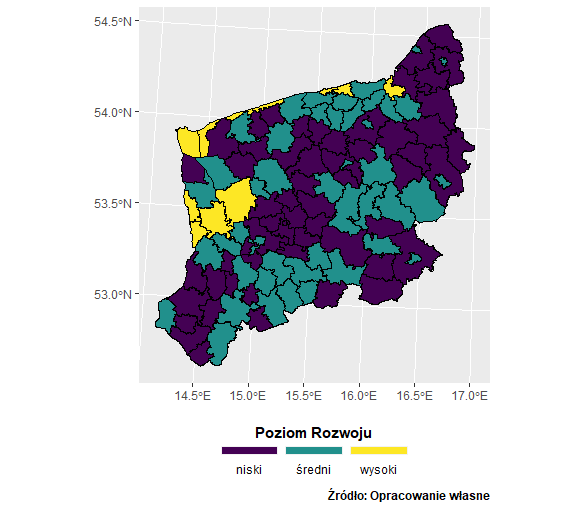
\includegraphics[width=1\linewidth]{figures/mapa_2016_bez} 

}

\caption{Poziom rozwoju gmin w województwie Zachodniopomorskim (2016)}\label{fig:rycina6}
\end{figure}

W 2016 roku (patrz Rysunek \ref{fig:rycina6}) wysokim poziomem rozwoju charakteryzował się Szczecin wraz z~pobliskim gminami- Dobrą Szczecińską Kołbaskowem i~Goleniowem oraz miejscowości nabrzeżne- Świnoujście, Kołobrzeg, Mielno, Ustronie Morskie, Międzyzdroje, Dziwnów, Rewal. Drugim ośrodkiem miejskim nie należącym ani do aglomeracji Szczecińskiej ani nie będący gminą nadmorską, a~charakteryzujący się wysokim poziomem rozwoju jest Koszalin.
Koszalin oraz Kołobrzeg są gminami na północy województwa, których wysoki poziom rozwoju „dyfuzyjnie" rozchodzi się na powiat, tworząc razem z~Białogardem (większy ośrodek miejski, zakwalifikowany jako gmina o~średnim poziomie rozwoju) pas gmin o~średnim poziomie rozwoju.
Scharakteryzować można pas gmin o~niskim poziomie rozwoju ciągnący się pojezierzem zachodniopomorskim oraz gminy na wschód i~południe od Koszalina.

\begin{figure}[t]

{\centering 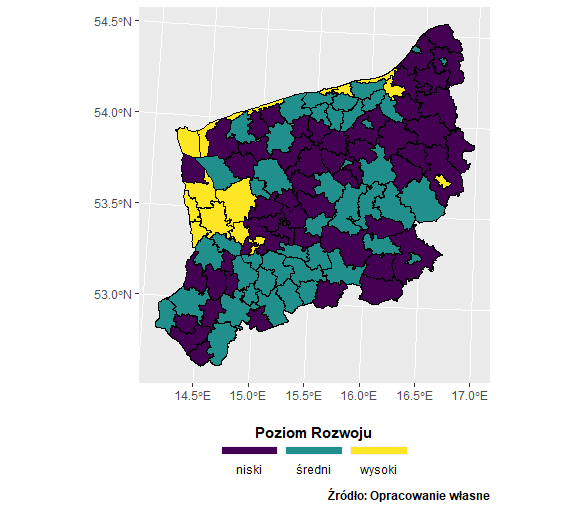
\includegraphics[width=1\linewidth]{figures/mapa_2017_bez} 

}

\caption{Poziom rozwoju gmin w województwie Zachodniopomorskim (2017)}\label{fig:rycina7}
\end{figure}

W 2017 roku (patrz Rysunek \ref{fig:rycina7}) widać przyrost gmin charakteryzujących się wysokim poziomem rozwoju w obrębie aglomeracji szczecińskiej.
W porównaniu do roku poprzedniego do kategorii tej dołączył Stargard, Police, Kobylanka.
Koszalin oraz miejscowości nadmorskie także zostały przydzielone do wysokiego poziomu rozwoju.
Natomiast ciekawym przypadkiem jest miasto Szczecinek, które w 2017 roku osiągnęło wysoki poziom rozwoju społeczno-gospodarczego, a okola je gmina wiejska o takiej samej nazwie charakteryzująca się niskim poziomem rozwoju.
Gminy w powiecie stargardzkim (Dolice, Suchań) odznaczają się średnim poziomem rozwoju.
Generalizując jest to rok „lepszy" dla gmin w zachodniej części województwa.

\begin{figure}[t]

{\centering 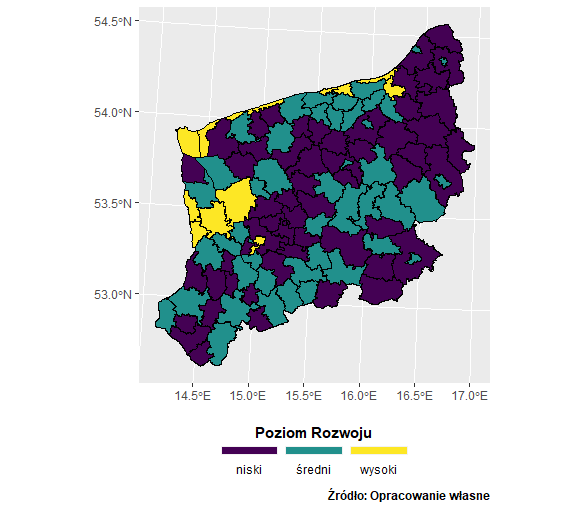
\includegraphics[width=1\linewidth]{figures/mapa_2018_bez} 

}

\caption{Poziom rozwoju gmin w województwie Zachodniopomorskim (2018)}\label{fig:rycina8}
\end{figure}

W 2018 (patrz Rysunek \ref{fig:rycina8}) roku Police oraz Kobylanka przydzielone zostały do gmin o średnim poziomie rozwoju. Można powiedzieć, że aglomeracja Szczecińska „osłabła``, jednak Stargard pozostał gminą o wysokim poziomie rozwoju. Warto zaznaczyć, że jest to największy ośrodek miejski w aglomeracji Szczecińskiej oprócz Szczecina.
Miasto Szczecinek tak jak w 2016 roku zostało sklasyfikowane jako gmina o~średnim poziomie rozwoju.
Dolice, Lipiany i Suchań ponownie „wróciły'' do gmin o niskim poziomie rozwoju.

\begin{figure}[t]

{\centering 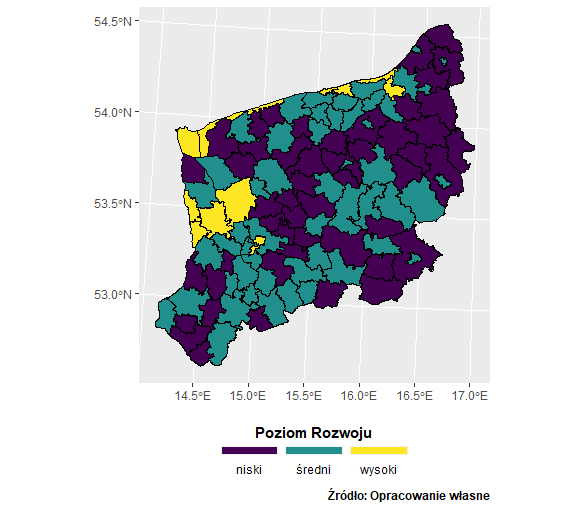
\includegraphics[width=1\linewidth]{figures/mapa_2019_bez} 

}

\caption{Poziom rozwoju gmin w województwie Zachodniopomorskim (2019)}\label{fig:rycina9}
\end{figure}

Brak zmian wśród gmin o wysokim poziomie rozwoju w 2019 roku (patrz Rysunek \ref{fig:rycina9}) w stosunku do roku poprzedniego. Widać pozytywny wpływ Stargardu, który pozostał jako gmina o~wysokim poziomie rozwoju i~wpłynął na okalającej miasto gminę wiejską o~tej samej nazwie.
Gmina miejsko-wiejska Sianów na wschód od Koszalina zaklasyfikowała się jako gmina o~średnim poziomie rozwoju.

\begin{verbatim}
#> tweaking randomForest
\end{verbatim}

\hypertarget{podsumowanie1}{%
\chapter{Podsumowanie}\label{podsumowanie1}}

W pracy potwierdzono, że metoda k-średnich jest dobrym narzędziem dla stosunkowo niewielkiej liczby obserwacji (114).
Przedstawiono pomocne metody wyliczenia optymalnej liczby skupień.
W pracy zdecydowano się na 3 skupienia, jednak opierając się na metodach wyboru optymalnej liczby skupień ciekawe byłyby dalsze badania oparte na 4 lub 5 skupieniach.

Badanie poziomu istotności czynników podczas klasyfikacji pokazało jak istotna dla poziomu rozwoju jest zwarta tkanka przestrzenna, która ujęta została w takich czynnikach jak \emph{udział osób korzystających z instalacji gazowej w ogóle populacji {[}\%{]}}, \emph{\%~mieszkań posiadających centralne ogrzewanie}, \emph{różnica pomiędzy odsetkiem ludności korzystającej z wodociągu i z kanalizacji} oraz \emph{dochody z podatku rolnego na 1 mieszkańca {[}zł{]}}.
Prócz powyższych istotny wpływ na poziom rozwoju mają „twarde" wskaźniki dotyczące życia gospodarczego takie jak \emph{osoby fizyczne prowadzące działalność gospodarczą na 1000 ludności}, \emph{podmioty gospodarcze w sekcjach J-N (usługi, specjaliści, informatyka) na 1000 mieszkańców}, \emph{pracujący na 1000 osób w wieku produkcyjnym}.
Zgodnie z badaniami dominującym aspektem poziomu rozwoju jest kapitał materialny, a~za nim kapitał finansowy.
Warto zauważyć duże znaczenie innowacji na rozwój, bowiem mimo stosunkowo małego wpływu na poziom rozwoju to był on wyższy lub porównywalny od kapitału społecznego oraz ludzkiego i to pomimo jedynie dwóch wskaźników jakie przekładały się na poziom innowacji.
Pokazało to, że słusznym okazało się zawarcie do danych dotyczących podmiotów gospodarczych w sekcjach J-N (usługi, specjaliści, informatyka) na 1000 mieszkańców do wskaźników zaproponowanych przez Pana Doktora Perdała (\textcite{perdal_zastosowanie}).

Dalszych badań wymaga dobór danych do konstrukcji syntetycznego wskaźnika rozwoju, bowiem jak zauważono w badaniu istotny wpływ na poziom rozwoju ma jedynie część z dobranych wskaźników.
Należałoby zwłaszcza przyjrzeć się innym możliwym wskaźnikom mogącym składać się na poziom innowacyjności.
Możliwe, że część otrzymanych wyników dotyczących istotności badanych wskaźników wynika ze specyfikacji województwa Zachodniopomorskiego, dlatego w dalszych badaniach należałoby objąć cały kraj.

Jednoczynnikowa analiza wariancji pozwoliła prześledzić polaryzacje poziomu rozwoju gmin w województwie Zachodniopomorskim.
Na przestrzeni lat 2016-2019 ustalono, że różnica między średnim poziomem rozwoju i wysokim jest znacząco wyższa niż między średnim poziomem rozwoju i niskim.
Świadczy to o rosnącej dysproporcji w poziomie rozwoju gmin.
Dzięki temu ustalono, że między rokiem 2016, a 2017 różnica między poszczególnymi poziomami rozwoju znacząco spadła.
Natomiast w roku 2018, 2019 polaryzacja poziomu rozwoju wzrastała.
Różnica poziomów rozwoju w 2019 roku była wyższa niż w 2016.

Zaobserwowano także jak niezwykle wszechstronne jest środowisko R. Dzięki mnogości pakietów, pozwala zarówno na transformacje, eksploracje, analizę danych jak i~również daje narzędzia do wizualizacji przestrzennej.
Czyni to środowisko R użytecznym narzędziem do badań nad poziomem rozwoju społeczno-gospodarczym.

\printbibliography[heading=bibintoc, title=Bibliografia]

\end{document}
